\documentclass[
  12pt,
  openany,
  oneside,
  a4paper,
  brazilian
]{abntex2}

% ==============================================================================
% CONFIGURAÇÃO EM CONFORMIDADE COM O MANUAL DE NORMALIZAÇÃO DA UFAL (2022)
% ==============================================================================

% --- Margens Oficiais (Manual UFAL p. 19-20 / NBR 14724) ---
% Superior: 3 cm, Esquerda: 3 cm, Inferior: 2 cm, Direita: 2 cm
\usepackage[
  a4paper,
  top=3cm,
  left=3cm,
  bottom=2cm,
  right=2cm,
  headheight=15pt,
  footskip=1cm
]{geometry}

% --- Tipografia Oficial (Manual UFAL p. 19 / NBR 14724) ---
% Times New Roman com suporte matemático completo e Courier escalado
\usepackage{cmap}
\usepackage[T1]{fontenc}
\usepackage[utf8]{inputenc}
\usepackage{newtxtext,newtxmath}
\usepackage[scaled=0.90]{couriers}

% --- Espaçamentos Oficiais (Manual UFAL p. 21) ---
% Entrelinhas de 1,5 cm no corpo do texto; simples para citações longas e notas
\usepackage{setspace}
\OnehalfSpacing
\setlength{\parindent}{1.25cm}
\setlength{\parskip}{0pt}

% --- Pacotes Auxiliares Essenciais ---
\usepackage{indentfirst}
\usepackage{color}
\usepackage{xcolor}
\usepackage{graphicx}
\usepackage{microtype}
\usepackage{amsmath}
\usepackage{booktabs}
\usepackage{longtable}
\usepackage{array}
\usepackage{colortbl}
\usepackage{listings}
\usepackage{tikz}
\usetikzlibrary{shapes.geometric, arrows.meta, positioning, calc, fit, backgrounds}
\usepackage{hyperref}

% --- Padronização dos Títulos conforme NBR 6024 e Manual UFAL p. 49-51 ---
% Seção Primária: MAIÚSCULAS e NEGRITO
% Seção Secundária: Negrito, apenas inicial maiúscula
% Seção Terciária: Não negritada (regular), apenas inicial maiúscula
\renewcommand{\ABNTEXchapterfont}{\rmfamily\bfseries}
\renewcommand{\ABNTEXchapterfontsize}{\normalsize\bfseries}
\renewcommand{\ABNTEXsectionfont}{\rmfamily\bfseries}
\renewcommand{\ABNTEXsectionfontsize}{\normalsize\bfseries}
\renewcommand{\ABNTEXsubsectionfont}{\rmfamily\normalfont}
\renewcommand{\ABNTEXsubsectionfontsize}{\normalsize\normalfont}
\renewcommand{\ABNTEXsubsubsectionfont}{\rmfamily\itshape}
\renewcommand{\ABNTEXsubsubsectionfontsize}{\normalsize\itshape}
\renewcommand{\familydefault}{\rmdefault}

% Configurações no Sumário (Manual UFAL p. 51)
\renewcommand{\cftchapterfont}{\bfseries}
\renewcommand{\cftchapterpagefont}{\bfseries}
\renewcommand{\cftsectionfont}{\bfseries}
\renewcommand{\cftsectionpagefont}{\bfseries}
\renewcommand{\cftsubsectionfont}{\normalfont}
\renewcommand{\cftsubsectionpagefont}{\normalfont}

% Oculta o título interno do sumário para usar o título centralizado oficial
\renewcommand{\printtoctitle}[1]{}

% Título de Referências centralizado conforme Manual UFAL p. 21
\renewcommand{\bibname}{REFERÊNCIAS}

% --- Configurações Limpas do Listings ---
\definecolor{codegreen}{rgb}{0,0.5,0}
\definecolor{codegray}{rgb}{0.45,0.45,0.45}
\definecolor{codepurple}{rgb}{0.5,0,0.7}
\definecolor{backcolour}{rgb}{0.98,0.98,0.98}

\lstdefinestyle{mystyle}{
    backgroundcolor=\color{backcolour},   
    commentstyle=\color{codegreen}\itshape,
    keywordstyle=\color{blue!80!black}\bfseries,
    numberstyle=\tiny\color{codegray},
    stringstyle=\color{codepurple},
    basicstyle=\ttfamily\footnotesize,
    breakatwhitespace=false,         
    breaklines=true,                 
    captionpos=b,                    
    keepspaces=true,                 
    numbers=none,                    
    showspaces=false,                
    showstringspaces=false,
    showtabs=false,                  
    tabsize=2,
    frame=lines,
    rulecolor=\color{gray!40}
}
\lstset{style=mystyle}

% --- Configurações de hiperlinks discretos ---
\hypersetup{
    colorlinks=true,
    linkcolor=black,
    citecolor=black,
    filecolor=black,      
    urlcolor=blue!75!black
}

% --- Definição de subtítulo ---
\newcommand{\subtitulo}[1]{\newcommand{\imprimirsubtitulo}{#1}}

% --- Informações Institucionais ---
\titulo{DESENVOLVIMENTO DE UM COMPILADOR MINIPAR 2026.2}
\autor{Érico Almeida Bernardino \and Felipe Lima Aragão \and Lucas Trindade de Souza}
\local{Maceió, AL}
\data{2026}

% ==============================================================================
% INÍCIO DO DOCUMENTO
% ==============================================================================
\begin{document}

\shorthandoff{"}
\frenchspacing

% ==============================================================================
% ELEMENTOS PRÉ-TEXTUAIS (Manual UFAL p. 19-25)
% ==============================================================================
\pagestyle{empty}

% --- 1. CAPA OFICIAL (Manual UFAL Figura 6 e 7, p. 24-25) ---
\begin{capa}
    \centering
    {\ABNTEXchapterfont\bfseries\normalsize UNIVERSIDADE FEDERAL DE ALAGOAS}\\[0.2cm]
    {\ABNTEXchapterfont\bfseries\normalsize INSTITUTO DE COMPUTAÇÃO}\\[0.2cm]
    {\ABNTEXchapterfont\bfseries\normalsize CIÊNCIA DA COMPUTAÇÃO}

    \vspace{3.5cm}

    {\normalsize\bfseries ÉRICO ALMEIDA BERNARDINO}\\[0.2cm]
    {\normalsize\bfseries FELIPE LIMA ARAGÃO}\\[0.2cm]
    {\normalsize\bfseries LUCAS TRINDADE DE SOUZA}

    \vspace{4.0cm}

    {\ABNTEXchapterfont\bfseries\normalsize DESENVOLVIMENTO DE UM COMPILADOR PARA A LINGUAGEM MINIPAR 2026.2}\\[0.6cm]
    {\normalsize\url{https://github.com/Felipe-Aragao/Minipar2026.2}}

    \vfill
    {\normalsize\bfseries MACEIÓ -- AL}\\[0.2cm]
    {\normalsize\bfseries 2026}
\end{capa}

% --- 2. SUMÁRIO (Manual UFAL p. 51 - Palavra SUMÁRIO centralizada) ---
\clearpage
\pdfbookmark[0]{\contentsname}{toc}
\begin{center}
    {\ABNTEXchapterfont\bfseries\normalsize SUMÁRIO}
\end{center}
\vspace{0.5cm}
\tableofcontents*
\clearpage

% ==============================================================================
% ELEMENTOS TEXTUAIS (Manual UFAL p. 21 / NBR 14724)
% Numeração arábica a partir da Introdução no canto superior direito
% ==============================================================================
\textual
\pagestyle{simple}

\chapter{INTRODUÇÃO}

Este relatório técnico documenta a concepção, modelagem arquitetural, implementação e validação experimental do compilador para a linguagem MiniPar 2026.2, desenvolvido no âmbito da disciplina de Compiladores ministrada pelo Prof. Dr. Arturo Hernandez Dominguez no Instituto de Computação da Universidade Federal de Alagoas (UFAL).

A linguagem MiniPar é uma linguagem educacional projetada para explorar conceitos avançados de compilação, orientação a objetos e execução concorrente e distribuída. O MiniPar 2026.2 adota um pipeline estático composto por análise léxica, análise sintática com geração de Árvore de Sintaxe Abstrata (AST), análise semântica com verificação de tipos e escopos, motor de otimização independente de máquina na AST, síntese de Código Intermediário de Três Endereços (TAC) e transpilação para C++ nativo (padrão ISO C++20), gerando binários executáveis (\texttt{.exe}) compilados pelo \texttt{g++} com a flag \texttt{-O3}.

O compilador é fundamentado na versão anterior MiniPar 2026.1, sobre a qual foram adicionadas novas funcionalidades e componentes estruturais para atender integralmente às exigências da disciplina:

\begin{itemize}
    \item Arquitetura Baseada em Componentes (CBSE): desacoplamento de todas as etapas em componentes formais com interfaces abstratas no diretório \texttt{src/} (\texttt{componente\_lexico.py}, \texttt{componente\_sintatico.py}, \texttt{componente\_semantico.py}, \texttt{componente\_tabela\_simbolos.py}, \texttt{componente\_otimizador.py}, \texttt{componente\_tac.py} e \texttt{componente\_codegen.py});
    \item Primitivas de Real Paralelismo (\texttt{fork} e \texttt{join}): expansão dos analisadores léxico, sintático, semântico e do gerador de TAC para divisão explícita de tarefas em núcleos locais (\texttt{core}) ou nós remotos (\texttt{host}), com barreira de sincronização;
    \item Afinidade de Núcleos de Hardware e Runtime C++: chamadas nativas de sistema operacional em \texttt{src/cpp\_template.py} (\texttt{SetThreadAffinityMask} na API Win32 e \texttt{pthread\_setaffinity\_np} em POSIX/Linux) e pool assíncrono com \texttt{std::shared\_future};
    \item Motor de Otimização no Backend: módulo \texttt{src/optimizer.py} para simplificações algébricas, dobra de constantes (\textit{constant folding}) e eliminação de código morto na AST;
    \item Segunda Interface Web Didática: interface em \texttt{templates/didatico.html} com visualizador gráfico interativo da AST em SVG/D3.js, controles individuais para cada fase da compilação e suporte a entradas pré-digitadas no console;
    \item Suíte e Orquestrador dos 11 Testes Oficiais: validação dos 11 programas oficiais da disciplina, cobrindo cálculo de Speedup com multiprocessamento, renderização de fractais (Mandelbrot e Tapete de Sierpinski em BMP) e um mini-compilador com emissão de Assembly ARMv7 no Teste 11.
\end{itemize}

\section{Objetivos do Projeto}

O trabalho cumpre os requisitos da especificação oficial do projeto MiniPar 2026.2, assegurando:
\begin{enumerate}
    \item Corretude e Confiabilidade: compilação e execução estável dos 11 testes oficiais e aprovação total na suíte automatizada de testes;
    \item Rigor de Engenharia de Software: modelagem formal da arquitetura em diagramas UML de Casos de Uso, Componentes de Software (interfaces fornecidas e requeridas), Classes Conceituais e Atividades/Fluxo;
    \item Didática e Usabilidade: disponibilização de interfaces acessíveis tanto para desenvolvedores quanto para estudantes em aprendizado de compiladores.
\end{enumerate}

\section{Arquitetura Geral do Pipeline de Compilação}

A Tabela \ref{tab:arquitetura_geral} resume a estrutura arquitetural dos módulos do sistema, detalhando suas responsabilidades, arquivos de implementação e interfaces associadas.

\begin{table}[htbp]
\centering
\caption{Mapeamento da Arquitetura Geral do Compilador MiniPar 2026.2}
\label{tab:arquitetura_geral}
\small
\begin{tabular}{p{3.2cm}p{3.8cm}p{2.8cm}p{5cm}}
\toprule
Componente & Arquivo de Implementação & Interface (CBSE) & Responsabilidade Principal \\
\midrule
Entrada CLI & \texttt{main.py} & CLI / Dispatcher & Ponto de entrada, orquestração de flags (\texttt{-O}) e seletor de modo interativo. \\
Menu Terminal & \texttt{menu.py} & Console UI & Execução individual ou em lote dos 11 testes oficiais. \\
Servidor Web Flask & \texttt{app.py} & Web REST API & Disponibiliza a IDE Desenvolvedor (\texttt{/ide}) e a Didática (\texttt{/}). \\
Analisador Léxico & \texttt{src/lexer.py} & \texttt{ILexico} & Converte texto-fonte em tokens com linha e coluna, descartando comentários \texttt{\#}. \\
Analisador Sintático & \texttt{src/parser.py} & \texttt{ISintatico} & Constrói a AST com nós orientados a objetos via descida recursiva. \\
Nós da AST & \texttt{src/ast\_nodes.py} & Dataclasses & Modela nós sintáticos e oferece serialização JSON via \texttt{to\_dict()}. \\
Tabela de Símbolos & \texttt{src/componente\_tabela\_simbolos.py} & \texttt{ITabelaSimbolos} & Controla a pilha de escopos, variáveis, atributos e métodos. \\
Analisador Semântico & \texttt{src/semantic.py} & \texttt{ISemantico} & Validação estática de tipos, escopos, classes, herança e laços. \\
Otimizador AST & \texttt{src/optimizer.py} & \texttt{IOtimizador} & Backend: dobra de constantes, simplificação algébrica e código morto na AST. \\
Gerador de TAC & \texttt{src/tac.py} & \texttt{ITAC} & Síntese de código linear de 3 endereços com temporários e labels. \\
Gerador de C++ & \texttt{src/codegen.py} & \texttt{ICodegen} & Transpila AST validada para C++20 nativo e invoca o \texttt{g++ -O3}. \\
Runtime C++ & \texttt{src/cpp\_template.py} & Header nativo C++ & Threads, sockets TCP, afinidade de CPU e barreira de sincronização. \\
Análise Web & \texttt{src/analise.py} & Engine Modular & Executa o pipeline passo a passo em memória para a interface didática. \\
Orquestrador Multi-Terminal & \texttt{test\_orchestrator.py} & Sockets / JSON & Coordena terminais participantes em testes distribuídos. \\
\bottomrule
\end{tabular}
\end{table}

\chapter{A LINGUAGEM MINIPAR 2026.2 E GRAMÁTICA BNF}

A linguagem MiniPar 2026.2 é uma linguagem imperativa, concorrente, distribuída e fortemente tipada em seu modelo conceitual, integrando elementos sintáticos inspirados em Python, C++ e Go. Sua gramática formal suporta abstrações para Orientação a Objetos, controle de fluxo abrangente, manipulação de coleções dinâmicas e estruturas para comunicação e paralelismo.

\section{Características Fundamentais e Novos Paradigmas}

O compilador dá suporte formal ao paradigma de real paralelismo com execução em múltiplos núcleos e nós de rede:

\begin{enumerate}
    \item Blocos \texttt{seq} e \texttt{par}:
    O comando \texttt{seq \{ ... \}} garante a ordem sequencial de execução dos enunciados internos. O bloco \texttt{par \{ ... \}} dispara os comandos contidos como threads concorrentes no computador local, aguardando que todas concluam antes de prosseguir.
    
    \item Primitivas \texttt{fork} e \texttt{join} (Paralelismo Real Distribuído):
    A primitiva \texttt{fork} realiza a divisão de uma tarefa em subtarefas independentes alocadas explicitamente a recursos de processamento:
    \begin{itemize}
        \item \texttt{fork core(id) comando;} ou \texttt{fork core(id) \{ ... \}}: realiza a alocação determinística da subtarefa a um núcleo de CPU do processador local, isolando sua execução via afinidade de hardware (\textit{Core Affinity}).
        \item \texttt{fork host(ip, porta) comando;}: despacha e agenda a tarefa para execução em um computador remoto via rede.
    \end{itemize}
    A primitiva complementar \texttt{join} implementa a barreira de sincronização e coleta de dados:
    \begin{itemize}
        \item \texttt{join;} : aguarda o término de todas as tarefas disparadas pelo pool local.
        \item \texttt{join(t1, t2, ...);} : bloqueia a execução até que as tarefas indicadas concluam e disponibilizem seus resultados.
    \end{itemize}

    \item Comunicação por Mensagens via Canais (\texttt{c\_channel}):
    A troca de dados entre processos independentes ocorre por passagem de mensagens utilizando canais sobre sockets TCP/IP:
    \begin{itemize}
        \item Declaração: \texttt{var canal = c\_channel("127.0.0.1", 5000);}
        \item Envio: \texttt{send(canal, mensagem);}
        \item Recepção: \texttt{var dado = receive(canal);}
    \end{itemize}

    \item Orientação a Objetos Plena:
    Suporte completo a classes (\texttt{class}), herança simples (\texttt{extends}), instanciação explícita (\texttt{new}), referência à própria instância (\texttt{this}), construtores parametrizados e métodos com passagem de parâmetros.
\end{enumerate}

\section{Gramática Formal em Notação EBNF}

A sintaxe formal completa do MiniPar 2026.2 é descrita na notação BNF Estendida (EBNF), na qual \texttt{\{ x \}} denota zero ou mais repetições, \texttt{[ x ]} denota elemento opcional e \texttt{"token"} representa símbolo terminal.

\subsection{Estrutura Global do Programa}
\begin{lstlisting}[language=bash, caption={Produções globais e declarações}]
<programa> ::= { <declaracao> | <comando> }

<declaracao> ::= <declaracao_classe>
               | <declaracao_funcao>
               | <declaracao_variavel>

<declaracao_classe> ::= "class" <IDENTIFIER> [ "extends" <IDENTIFIER> ] "{" 
                          { <membro_classe> } 
                        "}"

<membro_classe> ::= <declaracao_variavel>
                  | <declaracao_funcao>

<declaracao_funcao> ::= "func" <IDENTIFIER> "(" [ <lista_parametros> ] ")" <bloco_comandos>

<lista_parametros> ::= <IDENTIFIER> { "," <IDENTIFIER> }

<declaracao_variavel> ::= ( "var" | <tipo> ) <IDENTIFIER> [ "=" <expressao> ] ";"
\end{lstlisting}

\subsection{Comandos e Estruturas de Controle}
\begin{lstlisting}[language=bash, caption={Produções de comandos e controle de fluxo}]
<comando> ::= <bloco_comandos>
            | <bloco_seq>
            | <bloco_par>
            | <comando_fork>
            | <comando_join>
            | <comando_if>
            | <comando_while>
            | <comando_do_while>
            | <comando_for>
            | <comando_print>
            | <comando_send>
            | <comando_return>
            | <comando_break>
            | <comando_continue>
            | <atribuicao> ";"
            | <chamada_metodo> ";"
            | <chamada_funcao> ";"

<bloco_comandos> ::= "{" { <comando> } "}"
<bloco_seq>      ::= "seq" "{" { <comando> } "}"
<bloco_par>      ::= "par" "{" { <comando> } "}"

<comando_fork>   ::= "fork" <destino> ( <bloco_comandos> | <expressao> ";" )
<destino>        ::= "core" "(" <expressao> ")" 
                   | "host" "(" <expressao> [ "," <expressao> ] ")"

<comando_join>   ::= "join" [ "(" [ <lista_expressoes> ] ")" ] ";"

<comando_if>     ::= "if" "(" <expressao> ")" <comando> [ "else" <comando> ]

<comando_while>  ::= "while" "(" <expressao> ")" <comando>

<comando_do_while> ::= "do" <comando> "while" "(" <expressao> ")" ";"

<comando_for>    ::= "for" "(" ( <for_tradicional> | <for_in> ) ")" <comando>
<for_tradicional> ::= [ <declaracao_variavel> | <atribuicao> ] ";" 
                      [ <expressao> ] ";" 
                      [ <atribuicao> | <expressao> ]
<for_in>          ::= "var" <IDENTIFIER> "in" <expressao>

<comando_print>  ::= "print" "(" [ <lista_expressoes> ] ")" ";"
<comando_send>   ::= "send" "(" <expressao> "," <expressao> ")" ";"
<comando_return> ::= "return" [ <expressao> ] ";"
<comando_break>  ::= "break" ";"
<comando_continue> ::= "continue" ";"
\end{lstlisting}

\subsection{Expressões e Precedência de Operadores}
\begin{lstlisting}[language=bash, caption={Hierarquia sintática de expressões}]
<expressao> ::= <expressao_logica_ou>

<expressao_logica_ou> ::= <expressao_logica_e> { "||" <expressao_logica_e> }

<expressao_logica_e>  ::= <expressao_igualdade> { "&&" <expressao_igualdade> }

<expressao_igualdade> ::= <expressao_relacional> { ( "==" | "!=" ) <expressao_relacional> }

<expressao_relacional> ::= <expressao_aditiva> { ( "<" | "<=" | ">" | ">=" ) <expressao_aditiva> }

<expressao_aditiva>   ::= <expressao_multiplicativa> { ( "+" | "-" ) <expressao_multiplicativa> }

<expressao_multiplicativa> ::= <expressao_unaria> { ( "*" | "/" | "%" ) <expressao_unaria> }

<expressao_unaria>    ::= ( "-" | "!" ) <expressao_unaria> | <expressao_posfixa>

<expressao_posfixa>   ::= <expressao_primaria> { 
                            "." <IDENTIFIER> [ "(" [ <lista_expressoes> ] ")" ]
                          | "[" <expressao> "]" 
                        }

<expressao_primaria>  ::= <NUMBER>
                        | <STRING_LITERAL>
                        | <BOOL_LITERAL>
                        | <IDENTIFIER>
                        | "this"
                        | "new" <IDENTIFIER> "(" [ <lista_expressoes> ] ")"
                        | "c_channel" "(" <expressao> "," <expressao> ")"
                        | "receive" "(" <expressao> ")"
                        | "input" "(" [ <expressao> ] ")"
                        | "matrix" "(" <expressao> "," <expressao> "," <expressao> ")"
                        | "[" [ <lista_expressoes> ] "]"
                        | "(" <expressao> ")"
                        | <comando_fork>
                        | <comando_join>
\end{lstlisting}

\chapter{ANALISADOR LÉXICO (LEXER)}

O Analisador Léxico (\textit{Lexer}) é o primeiro estágio do front-end do compilador MiniPar 2026.2, implementado no arquivo \texttt{src/lexer.py} e encapsulado no componente \texttt{C\_Lexico} que realiza a interface \texttt{ILexico}.

Sua responsabilidade é varrer sequencialmente o fluxo de caracteres do código-fonte e convertê-lo em uma lista linear de objetos estruturados da classe \texttt{Token}, na qual cada token carrega seu tipo categórico (\texttt{TokenType}), o lexema correspondente em texto, o número da linha de ocorrência e a coluna exata.

\section{Tratamento de Comentários, Delimitadores e Literais}

O analisador léxico incorpora regras robustas para garantir que construções complexas sejam extraídas sem ambiguidades:
\begin{itemize}
    \item Filtragem de Comentários (\texttt{\#}): ao encontrar o caractere cerquilha (\texttt{\#}) fora de literais de texto, o analisador consome todos os caracteres até a quebra de linha (\texttt{\textbackslash n}) ou o fim do arquivo. Isso assegura que anotações e comentários não interfiram nas fases sintáticas posteriores.
    \item Rastreamento Espacial: o contador de linha inicia em 1 e é incrementado a cada \texttt{\textbackslash n}. A coluna é atualizada a cada caractere lido e reiniciada após quebras de linha.
    \item Literais Numéricos e Ponto Flutuante: reconhece inteiros (\texttt{42}) e números decimais (\texttt{3.14159}), consumindo sequências de dígitos separadas por ponto.
    \item Literais de Texto e Escapes: delimitados por aspas duplas (\texttt{"..."}), com suporte a sequências de escape padrão (\texttt{\textbackslash n}, \texttt{\textbackslash t}, \texttt{\textbackslash "} e \texttt{\textbackslash\textbackslash}). O não fechamento das aspas dispara \texttt{LexError} com linha e coluna.
    \item Operadores Compostos: utiliza \textit{lookahead} de um caractere para diferenciar operadores simples de relacionais e lógicos compostos (\texttt{==}, \texttt{!=}, \texttt{<=}, \texttt{>=}, \texttt{\&\&} e \texttt{||}).
\end{itemize}

A Tabela \ref{tab:tokens_lexicos} resume as categorias de tokens reconhecidas pelo compilador.

\begin{table}[htbp]
\centering
\caption{Categorias e Exemplos de Tokens no MiniPar 2026.2}
\label{tab:tokens_lexicos}
\small
\begin{tabular}{p{3.5cm}p{11cm}}
\toprule
Categoria & Tokens Principais \\
\midrule
Palavras Reservadas & \texttt{class}, \texttt{extends}, \texttt{new}, \texttt{func}, \texttt{var}, \texttt{if}, \texttt{else}, \texttt{while}, \texttt{do}, \texttt{for}, \texttt{in}, \texttt{break}, \texttt{continue}, \texttt{return}, \texttt{seq}, \texttt{par}, \texttt{fork}, \texttt{join}, \texttt{core}, \texttt{host}, \texttt{this}, \texttt{c\_channel}, \texttt{send}, \texttt{receive}, \texttt{input}, \texttt{print}, \texttt{matrix} \\
Tipos Nativos & \texttt{number}, \texttt{int}, \texttt{string}, \texttt{bool}, \texttt{void}, \texttt{list}, \texttt{dict}, \texttt{task} \\
Literais & \texttt{NUMBER}, \texttt{STRING\_LITERAL}, \texttt{BOOL\_LITERAL} (\texttt{true}, \texttt{false}), \texttt{IDENTIFIER} \\
Operadores & \texttt{+}, \texttt{-}, \texttt{*}, \texttt{/}, \texttt{\%}, \texttt{=}, \texttt{==}, \texttt{!=}, \texttt{!}, \texttt{\&\&}, \texttt{||}, \texttt{<}, \texttt{>}, \texttt{<=}, \texttt{>=} \\
Delimitadores & \texttt{(}, \texttt{)}, \texttt{\{}, \texttt{\}}, \texttt{[}, \texttt{]}, \texttt{.}, \texttt{;}, \texttt{,} \\
Especiais & \texttt{END\_OF\_FILE}, \texttt{UNKNOWN} (para caracteres não reconhecidos) \\
\bottomrule
\end{tabular}
\end{table}

\section{Pseudocódigo do Analisador Léxico}

O Algoritmo \ref{algo:lexer} formaliza o procedimento de tokenização adotado pelo MiniPar 2026.2, atendendo expressamente ao Requisito 3 da especificação.

\begin{lstlisting}[language=Python, caption={Pseudocódigo do Analisador Léxico (Lexer)}, label={algo:lexer}]
ALGORITMO ANALISE_LEXICA(codigo_fonte):
    posicao <- 0
    linha <- 1
    coluna <- 1
    tokens <- Lista_Vazia()

    ENQUANTO posicao < tamanho(codigo_fonte):
        # 1. Pular espacos em branco e tabulacoes
        ENQUANTO posicao < tamanho(codigo_fonte) E eh_espaco(codigo_fonte[posicao]):
            SE codigo_fonte[posicao] == '\n':
                linha <- linha + 1
                coluna <- 1
            SENAO:
                coluna <- coluna + 1
            posicao <- posicao + 1

        # 2. Descarte de comentarios iniciados por '#'
        SE posicao < tamanho(codigo_fonte) E codigo_fonte[posicao] == '#':
            ENQUANTO posicao < tamanho(codigo_fonte) E codigo_fonte[posicao] != '\n':
                posicao <- posicao + 1
                coluna <- coluna + 1
            CONTINUAR_PROXIMA_ITERACAO

        SE posicao >= tamanho(codigo_fonte):
            PARAR_LACO

        inicio_linha <- linha
        inicio_coluna <- coluna
        caractere <- codigo_fonte[posicao]

        # 3. Identificadores e Palavras Reservadas
        SE eh_letra(caractere) OU caractere == '_':
            lexema <- ""
            ENQUANTO posicao < tamanho(codigo_fonte) E (eh_alfanumerico(codigo_fonte[posicao]) OU codigo_fonte[posicao] == '_'):
                lexema <- lexema + codigo_fonte[posicao]
                posicao <- posicao + 1
                coluna <- coluna + 1
            
            tipo <- CONSULTAR_PALAVRAS_RESERVADAS(lexema)
            SE tipo == NULO:
                tipo <- TOKEN_IDENTIFICADOR
            ADICIONAR_TOKEN(tokens, tipo, lexema, inicio_linha, inicio_coluna)

        # 4. Numeros (Inteiros e Flutuantes)
        SENAO SE eh_digito(caractere):
            lexema <- ""
            ENQUANTO posicao < tamanho(codigo_fonte) E eh_digito(codigo_fonte[posicao]):
                lexema <- lexema + codigo_fonte[posicao]
                posicao <- posicao + 1
                coluna <- coluna + 1
            
            SE posicao < tamanho(codigo_fonte) E codigo_fonte[posicao] == '.':
                lexema <- lexema + '.'
                posicao <- posicao + 1
                coluna <- coluna + 1
                ENQUANTO posicao < tamanho(codigo_fonte) E eh_digito(codigo_fonte[posicao]):
                    lexema <- lexema + codigo_fonte[posicao]
                    posicao <- posicao + 1
                    coluna <- coluna + 1
            
            ADICIONAR_TOKEN(tokens, TOKEN_NUMERO, lexema, inicio_linha, inicio_coluna)

        # 5. Strings Literais e Caracteres de Escape
        SENAO SE caractere == '"':
            posicao <- posicao + 1  # Consome aspas de abertura
            coluna <- coluna + 1
            texto <- ""
            ENQUANTO posicao < tamanho(codigo_fonte) E codigo_fonte[posicao] != '"':
                SE codigo_fonte[posicao] == '\\':
                    posicao <- posicao + 1
                    coluna <- coluna + 1
                    SE posicao >= tamanho(codigo_fonte):
                        LANCAR_ERRO_LEXICO("String nao terminada", inicio_linha, inicio_coluna)
                    escape_char <- codigo_fonte[posicao]
                    texto <- texto + PROCESSAR_ESCAPE(escape_char)
                SENAO:
                    texto <- texto + codigo_fonte[posicao]
                posicao <- posicao + 1
                coluna <- coluna + 1
            
            SE posicao >= tamanho(codigo_fonte) OU codigo_fonte[posicao] != '"':
                LANCAR_ERRO_LEXICO("String nao terminada", inicio_linha, inicio_coluna)
            
            posicao <- posicao + 1  # Consome aspas de fechamento
            coluna <- coluna + 1
            ADICIONAR_TOKEN(tokens, TOKEN_STRING, texto, inicio_linha, inicio_coluna)

        # 6. Operadores Relacionais, Compostos e Delimitadores
        SENAO:
            simbolo <- AVANCAR_E_OBTER_CARACTERE()
            SE simbolo == '=' E ESPIAR_PROXIMO() == '=':
                AVANCAR(); ADICIONAR_TOKEN(tokens, TOKEN_IGUALDADE, "==", inicio_linha, inicio_coluna)
            SENAO SE simbolo == '!' E ESPIAR_PROXIMO() == '=':
                AVANCAR(); ADICIONAR_TOKEN(tokens, TOKEN_DIFERENTE, "!=", inicio_linha, inicio_coluna)
            SENAO SE simbolo == '<' E ESPIAR_PROXIMO() == '=':
                AVANCAR(); ADICIONAR_TOKEN(tokens, TOKEN_MENOR_IGUAL, "<=", inicio_linha, inicio_coluna)
            SENAO SE simbolo == '>' E ESPIAR_PROXIMO() == '=':
                AVANCAR(); ADICIONAR_TOKEN(tokens, TOKEN_MAIOR_IGUAL, ">=", inicio_linha, inicio_coluna)
            SENAO SE simbolo == '&' E ESPIAR_PROXIMO() == '&':
                AVANCAR(); ADICIONAR_TOKEN(tokens, TOKEN_E_LOGICO, "&&", inicio_linha, inicio_coluna)
            SENAO SE simbolo == '|' E ESPIAR_PROXIMO() == '|':
                AVANCAR(); ADICIONAR_TOKEN(tokens, TOKEN_OU_LOGICO, "||", inicio_linha, inicio_coluna)
            SENAO SE simbolo ESTA_NO_MAPA_SIMBOLOS_SIMPLES():
                ADICIONAR_TOKEN(tokens, MAPA_SIMBOLOS[simbolo], simbolo, inicio_linha, inicio_coluna)
            SENAO:
                ADICIONAR_TOKEN(tokens, TOKEN_DESCONHECIDO, simbolo, inicio_linha, inicio_coluna)

    ADICIONAR_TOKEN(tokens, TOKEN_FIM_ARQUIVO, "", linha, coluna)
    RETORNAR tokens
FIM_ALGORITMO
\end{lstlisting}

\chapter{ANALISADOR SINTÁTICO (PARSER)}

O Analisador Sintático (\textit{Parser}) é responsável por verificar se a sequência linear de tokens produzida pelo Lexer obedece estritamente às regras gramaticais da linguagem MiniPar 2026.2 e por estruturar essas informações em uma Árvore de Sintaxe Abstrata (AST).

No compilador MiniPar 2026.2, o analisador está implementado em \texttt{src/parser.py} e encapsulado no componente \texttt{C\_Sintatico}, que realiza a interface \texttt{ISintatico}. A AST resultante é composta por classes de nós fortemente tipadas, definidas em \texttt{src/ast\_nodes.py}.

\section{Método de Descida Recursiva e Precedência por Camadas}

O analisador utiliza a técnica de Análise Sintática Descendente Recursiva (\textit{Recursive Descent Parsing}):
\begin{itemize}
    \item Cada símbolo não-terminal da gramática BNF corresponde a uma função ou método dedicado na classe \texttt{Parser}.
    \item Para eliminar ambiguidades e respeitar a precedência matemática e lógica dos operadores sem recursão à esquerda, as expressões são tratadas em camadas estratificadas descendentes:
    \begin{center}
    \small
    $\text{Expressão} \;\longrightarrow\; \text{OU} \;\longrightarrow\; \text{E} \;\longrightarrow\; \text{Igualdade} \;\longrightarrow\; \text{Relacional}$ \\
    $\;\longrightarrow\; \text{Aditiva} \;\longrightarrow\; \text{Multiplicativa} \;\longrightarrow\; \text{Unária} \;\longrightarrow\; \text{Pós-fixa} \;\longrightarrow\; \text{Primária}$
    \end{center}
    \item Em caso de divergência entre o token esperado e o token lido, o método \texttt{\_consume} lança uma exceção \texttt{ParseError}, indicando a mensagem acompanhada da linha e coluna correspondentes.
\end{itemize}

\section{Tratamento dos Construtos \texttt{fork} e \texttt{join}}

Foram adicionadas produções no analisador sintático para o mapeamento das primitivas de paralelismo:
\begin{enumerate}
    \item Produção de \texttt{fork}: o método \texttt{\_parse\_fork()} identifica a palavra-chave \texttt{fork}, analisa o destino de alocação (\texttt{core(expressao)} ou \texttt{host(ip, porta)}) e constrói o nó \texttt{ForkStmt}, associando-o ao comando ou bloco correspondente.
    \item Produção de \texttt{join}: o método \texttt{\_parse\_join()} reconhece a barreira global de sincronização (\texttt{join;}) e a espera seletiva por tarefas específicas (\texttt{join(t1, t2);}), gerando a instância de \texttt{JoinStmt}.
\end{enumerate}

\section{Pseudocódigo do Analisador Sintático}

O Algoritmo \ref{algo:parser} apresenta o pseudocódigo formal do analisador sintático, cumprindo o Requisito 4 do projeto.

\begin{lstlisting}[language=Python, caption={Pseudocódigo do Analisador Sintático (Parser)}, label={algo:parser}]
CLASSE Parser:
    ATRIBUTOS:
        tokens: Lista de Tokens
        posicao: Inteiro <- 0

    METODO analisar_programa():
        programa <- Novo No Program()
        ENQUANTO token_atual().tipo != TOKEN_FIM_ARQUIVO:
            comando <- analisar_comando_ou_declaracao()
            SE comando != NULO:
                programa.adicionar_comando(comando)
        RETORNAR programa

    METODO consumir(tipo_esperado, mensagem_erro):
        SE token_atual().tipo == tipo_esperado:
            t <- token_atual()
            posicao <- posicao + 1
            RETORNAR t
        SENAO:
            LANCAR ParseError(mensagem_erro, token_atual().linha, token_atual().coluna)

    METODO analisar_comando_ou_declaracao():
        token <- token_atual()
        SE token.tipo == TOKEN_CLASS:
            RETORNAR analisar_declaracao_classe()
        SENAO SE token.tipo == TOKEN_FUNC:
            RETORNAR analisar_declaracao_funcao()
        SENAO SE token.tipo == TOKEN_VAR OU token.tipo == TOKEN_TIPO:
            RETORNAR analisar_declaracao_variavel()
        SENAO SE token.tipo == TOKEN_SEQ:
            RETORNAR analisar_bloco_seq()
        SENAO SE token.tipo == TOKEN_PAR:
            RETORNAR analisar_bloco_par()
        SENAO SE token.tipo == TOKEN_FORK:
            RETORNAR analisar_comando_fork()
        SENAO SE token.tipo == TOKEN_JOIN:
            RETORNAR analisar_comando_join()
        SENAO SE token.tipo == TOKEN_IF:
            RETORNAR analisar_comando_if()
        SENAO SE token.tipo == TOKEN_WHILE:
            RETORNAR analisar_comando_while()
        SENAO SE token.tipo == TOKEN_DO:
            RETORNAR analisar_comando_do_while()
        SENAO SE token.tipo == TOKEN_FOR:
            RETORNAR analisar_comando_for()
        SENAO SE token.tipo == TOKEN_PRINT:
            RETORNAR analisar_comando_print()
        SENAO SE token.tipo == TOKEN_SEND:
            RETORNAR analisar_comando_send()
        SENAO SE token.tipo == TOKEN_RETURN:
            RETORNAR analisar_comando_return()
        SENAO SE token.tipo == TOKEN_BREAK:
            consumir(TOKEN_BREAK, "Esperado 'break'"); consumir(TOKEN_PONTO_VIRGULA, "Esperado ';'")
            RETORNAR Novo No BreakStmt()
        SENAO SE token.tipo == TOKEN_CONTINUE:
            consumir(TOKEN_CONTINUE, "Esperado 'continue'"); consumir(TOKEN_PONTO_VIRGULA, "Esperado ';'")
            RETORNAR Novo No ContinueStmt()
        SENAO:
            expr <- analisar_expressao()
            SE token_atual().tipo == TOKEN_ATRIBUICAO:
                consumir(TOKEN_ATRIBUICAO, "Esperado '='")
                valor <- analisar_expressao()
                consumir(TOKEN_PONTO_VIRGULA, "Esperado ';'")
                RETORNAR Novo No Assignment(alvo=expr, valor=valor)
            consumir(TOKEN_PONTO_VIRGULA, "Esperado ';'")
            RETORNAR expr

    METODO analisar_comando_fork():
        consumir(TOKEN_FORK, "Esperado 'fork'")
        SE token_atual().tipo == TOKEN_CORE:
            consumir(TOKEN_CORE, "Esperado 'core'")
            consumir(TOKEN_ABRE_PARENTESES, "Esperado '('")
            nucleo <- analisar_expressao()
            consumir(TOKEN_FECHA_PARENTESES, "Esperado ')'")
            destino <- Novo No Destino(tipo="core", args=[nucleo])
        SENAO SE token_atual().tipo == TOKEN_HOST:
            consumir(TOKEN_HOST, "Esperado 'host'")
            consumir(TOKEN_ABRE_PARENTESES, "Esperado '('")
            host_ip <- analisar_expressao()
            consumir(TOKEN_VIRGULA, "Esperado ','")
            porta <- analisar_expressao()
            consumir(TOKEN_FECHA_PARENTESES, "Esperado ')'")
            destino <- Novo No Destino(tipo="host", args=[host_ip, porta])
        SENAO:
            LANCAR ParseError("Destino do fork deve ser 'core' ou 'host'", token_atual().linha)

        corpo <- analisar_comando_ou_declaracao()
        RETORNAR Novo No ForkStmt(destino=destino, corpo=corpo)

    METODO analisar_comando_join():
        consumir(TOKEN_JOIN, "Esperado 'join'")
        args <- Lista_Vazia()
        SE token_atual().tipo == TOKEN_ABRE_PARENTESES:
            consumir(TOKEN_ABRE_PARENTESES, "Esperado '('")
            SE token_atual().tipo != TOKEN_FECHA_PARENTESES:
                args.adicionar(analisar_expressao())
                ENQUANTO token_atual().tipo == TOKEN_VIRGULA:
                    consumir(TOKEN_VIRGULA, "Esperado ','")
                    args.adicionar(analisar_expressao())
            consumir(TOKEN_FECHA_PARENTESES, "Esperado ')'")
        consumir(TOKEN_PONTO_VIRGULA, "Esperado ';'")
        RETORNAR Novo No JoinStmt(args=args)

    METODO analisar_expressao():
        RETORNAR analisar_ou_logico()

    METODO analisar_ou_logico():
        esquerda <- analisar_e_logico()
        ENQUANTO token_atual().tipo == TOKEN_OU_LOGICO:
            op <- consumir(TOKEN_OU_LOGICO, "Esperado '||'").lexema
            direita <- analisar_e_logico()
            esquerda <- Novo No BinaryExpr(op=op, esquerda=esquerda, direita=direita)
        RETORNAR esquerda
FIM_CLASSE
\end{lstlisting}

\chapter{ANALISADOR SEMÂNTICO E TRATAMENTO DE ERROS}

O Analisador Semântico do compilador MiniPar 2026.2, implementado em \texttt{src/semantic.py} e operado através do componente \texttt{C\_Semantico} (interface \texttt{ISemantico}), é encarregado de verificar a consistência lógica, estrutural e tipológica da Árvore de Sintaxe Abstrata gerada pelo Parser.

\section{Estratégia de Duas Passagens (\textit{Two-Pass Analysis})}

Para permitir que funções e classes sejam utilizadas no código-fonte antes de suas declarações textuais (referência antecipada ou \textit{forward declaration}), o analisador adota um modelo de validação em duas etapas:
\begin{enumerate}
    \item Primeira Passagem (Coleta de Declarações): percorre a lista de comandos do nó raiz \texttt{Program} e registra todas as definições globais de classes (com métodos e atributos) e funções (com parâmetros formais) na Tabela de Símbolos. Caso haja duplicação de identificadores no mesmo escopo, um erro semântico é reportado.
    \item Segunda Passagem (Validação e Inferência de Tipos): inspeciona cada nó de comando e expressão, validando:
    \begin{itemize}
        \item Existência e visibilidade de variáveis acessadas em seus respectivos escopos;
        \item Compatibilidade estática e coerência em atribuições e operações binárias/unárias;
        \item Conformidade da quantidade de argumentos em chamadas de funções e métodos;
        \item Validação de contexto de fluxo: controle da profundidade de laços (\texttt{loop\_depth}), impedindo o uso indevido de \texttt{break} ou \texttt{continue} fora de blocos de repetição;
        \item Uso de \texttt{this} restrito ao escopo interno de métodos de classes;
        \item Tipagem de primitivas concorrentes (\texttt{fork} gera o tipo de tarefa \texttt{task}, e canais \texttt{c\_channel} operam com strings/números).
    \end{itemize}
\end{enumerate}

\section{Tratamento de Comentários (\texttt{\#}) e Diagnósticos de Erros}

O Requisito 5 especifica que o compilador deve permitir comentários via \texttt{\#}:
\begin{itemize}
    \item Os comentários são descartados na análise léxica, mantendo os contadores de linha e coluna perfeitamente sincronizados.
    \item Quando o Analisador Semântico detecta uma inconformidade (por exemplo, uso de variável não declarada), ele reporta o erro identificando a linha original do código MiniPar, desconsiderando linhas de comentários.
    \item A saída do erro é padronizada no formato:
    \[ \texttt{[ERRO SEMANTICO] Linha L, Coluna C: Mensagem Explicativa} \]
\end{itemize}

\section{Pseudocódigo do Analisador Semântico}

O Algoritmo \ref{algo:semantico} descreve a lógica e as rotinas de verificação do analisador semântico.

\begin{lstlisting}[language=Python, caption={Pseudocódigo do Analisador Semântico e Tratamento de Erros}, label={algo:semantico}]
CLASSE AnalisadorSemantico:
    ATRIBUTOS:
        tabela_simbolos: TabelaDeSimbolos
        erros: Lista de Erros <- []
        classes_declaradas: Mapa[Nome, MetadadosClasse]
        funcoes_declaradas: Mapa[Nome, MetadadosFuncao]
        profundidade_laco: Inteiro <- 0
        classe_atual: Texto <- NULO

    METODO reportar_erro(mensagem, linha, coluna):
        # Permite identificar erros ignorando comentarios ('#') filtrados pelo Lexer
        erro <- Novo Objeto Erro(fase="semantica", linha=linha, coluna=coluna, mensagem=mensagem)
        erros.adicionar(erro)
        IMPRIMIR("[ERRO SEMANTICO] Linha " + linha + ": " + mensagem)

    METODO analisar(programa):
        # Passagem 1: Coleta global de classes e funcoes
        PARA CADA declaracao EM programa.comandos:
            SE declaracao eh ClassDecl:
                SE declaracao.nome JA_EXISTE EM classes_declaradas:
                    reportar_erro("Classe '" + declaracao.nome + "' ja declarada", declaracao.linha)
                classes_declaradas[declaracao.nome] <- declaracao
            SENAO SE declaracao eh FuncDecl:
                SE declaracao.nome JA_EXISTE EM funcoes_declaradas:
                    reportar_erro("Funcao '" + declaracao.nome + "' ja declarada", declaracao.linha)
                funcoes_declaradas[declaracao.nome] <- declaracao

        # Passagem 2: Validacao de escopos e tipos
        PARA CADA comando EM programa.comandos:
            validar_no(comando)

        RETORNAR (tamanho(erros) == 0)

    METODO inferir_tipo(no):
        SE no eh NumberExpr: RETORNAR "number"
        SE no eh StringExpr: RETORNAR "string"
        SE no eh BoolExpr:   RETORNAR "bool"
        SE no eh ListLiteral: RETORNAR "list"
        SE no eh ForkStmt:   RETORNAR "task"
        SE no eh IdentifierExpr:
            simbolo <- tabela_simbolos.consultar(no.nome)
            SE simbolo != NULO: RETORNAR simbolo.tipo
            RETORNAR "unknown"
        SE no eh BinaryExpr:
            SE no.op EM ["==", "!=", "<", "<=", ">", ">=", "&&", "||"]:
                RETORNAR "bool"
            tipo_esq <- inferir_tipo(no.esquerda)
            tipo_dir <- inferir_tipo(no.direita)
            SE no.op == "+" E (tipo_esq == "string" OU tipo_dir == "string"):
                RETORNAR "string"
            RETORNAR "number"
        RETORNAR "unknown"

    METODO validar_no(no):
        SE no eh VarDecl:
            SE no.valor_inicial != NULO:
                validar_no(no.valor_inicial)
                tipo_valor <- inferir_tipo(no.valor_inicial)
                SE no.tipo != "var" E tipo_valor != "unknown" E no.tipo != tipo_valor:
                    reportar_erro("Tipo incompativel na inicializacao de '" + no.nome + "'", no.linha)
            declarou <- tabela_simbolos.declarar(no.nome, no.tipo, no.linha)
            SE NAO declarou:
                reportar_erro("Variavel '" + no.nome + "' ja declarada no escopo", no.linha)

        SENAO SE no eh Assignment:
            validar_no(no.valor)
            SE no.alvo eh IdentifierExpr:
                simbolo <- tabela_simbolos.consultar(no.alvo.nome)
                SE simbolo == NULO:
                    reportar_erro("Variavel '" + no.alvo.nome + "' nao declarada", no.linha)
                SENAO:
                    tipo_valor <- inferir_tipo(no.valor)
                    SE simbolo.tipo != "var" E tipo_valor != "unknown" E simbolo.tipo != tipo_valor:
                        reportar_erro("Atribuicao de tipo incompativel em '" + no.alvo.nome + "'", no.linha)

        SENAO SE no eh WhileStmt OU no eh DoWhileStmt:
            validar_no(no.condicao)
            profundidade_laco <- profundidade_laco + 1
            tabela_simbolos.entrar_escopo()
            validar_no(no.corpo)
            tabela_simbolos.sair_escopo()
            profundidade_laco <- profundidade_laco - 1

        SENAO SE no eh BreakStmt OU no eh ContinueStmt:
            SE profundidade_laco == 0:
                reportar_erro("Comando break/continue fora de laco de repeticao", no.linha)

        SENAO SE no eh SeqBlock OU no eh ParBlock:
            tabela_simbolos.entrar_escopo()
            PARA CADA subcomando EM no.comandos:
                validar_no(subcomando)
            tabela_simbolos.sair_escopo()

        SENAO SE no eh ForkStmt:
            validar_no(no.destino.args)
            validar_no(no.corpo)

        SENAO SE no eh JoinStmt:
            PARA CADA arg EM no.args:
                validar_no(arg)
FIM_CLASSE
\end{lstlisting}

\chapter{TABELA DE SÍMBOLOS}

A Tabela de Símbolos é a estrutura de dados central encarregada de registrar e consultar identificadores de variáveis, funções, classes, métodos e atributos declarados ao longo da compilação de um programa em MiniPar 2026.2. 

No compilador, a gestão de símbolos está formalizada no componente \texttt{C\_TabelaSimbolos} (\texttt{src/componente\_tabela\_simbolos.py}), que realiza os contratos da interface \texttt{ITabelaSimbolos}.

\section{Estrutura de Dados e Pilha de Escopos Léxicos}

A arquitetura adota uma Pilha de Dicionários de Símbolos (\textit{Scope Stack}):
\begin{itemize}
    \item Escopo Global: corresponde à base da pilha (índice 0), contendo as declarações acessíveis universalmente em todo o módulo compilado.
    \item Escopos Locais Aninhados: a cada entrada em um novo contexto delimitado (corpo de funções, métodos de classes, blocos de controle \texttt{if}, laços \texttt{while}/\texttt{for} e blocos concorrentes \texttt{seq}/\texttt{par}), uma nova tabela local é empilhada através da operação \texttt{entrar\_escopo()}.
    \item Resolução de Identificadores (Sombra / \textit{Shadowing}): a consulta (\texttt{consultar(nome)}) percorre a pilha em sentido descendente (do topo atual para a base). Se um símbolo existir em um escopo mais interno, ele tem prioridade sobre definições em escopos externos, modelando o sombreamento de variáveis.
    \item Encerramento de Escopo: ao atingir o término de um bloco, o método \texttt{sair\_escopo()} desempilha a tabela local. Para alimentar relatórios didáticos na interface Web, o componente preserva um histórico de todos os símbolos registrados na sessão.
\end{itemize}

Cada símbolo é modelado como uma instância da classe \texttt{Symbol}, registrando:
\begin{itemize}
    \item \texttt{name}: Nome textual do identificador;
    \item \texttt{type}: Tipo associado (\texttt{int}, \texttt{number}, \texttt{string}, \texttt{bool}, \texttt{list}, \texttt{task}, nome da classe ou \texttt{var});
    \item \texttt{params}: Lista de tipos/nomes de parâmetros (no caso de funções e métodos);
    \item \texttt{attributes}: Dicionário de atributos de instância com seus respectivos tipos;
    \item \texttt{methods}: Dicionário contendo as assinaturas de métodos declarados na classe.
\end{itemize}

\section{Pseudocódigo da Tabela de Símbolos}

O Algoritmo \ref{algo:tabela_simbolos} formaliza a implementação do componente de Tabela de Símbolos, atendendo ao Requisito 6.

\begin{lstlisting}[language=Python, caption={Pseudocódigo da Tabela de Símbolos}, label={algo:tabela_simbolos}]
CLASSE Simbolo:
    ATRIBUTOS:
        nome: Texto
        tipo: Texto
        parametros: Lista de Textos <- []
        atributos: Dicionario[Texto, Texto] <- {}
        metodos: Dicionario[Texto, Lista de Textos] <- {}

CLASSE TabelaDeSimbolos:
    ATRIBUTOS:
        pilha_escopos: Pilha de Dicionarios[Texto, Simbolo]
        historico_declaracoes: Lista de Metadados
        proximo_id_escopo: Inteiro <- 1

    METODO inicializar():
        pilha_escopos <- Nova_Pilha()
        escopo_global <- Novo_Dicionario()
        pilha_escopos.empilhar(escopo_global)

    METODO entrar_escopo():
        novo_escopo_local <- Novo_Dicionario()
        pilha_escopos.empilhar(novo_escopo_local)
        proximo_id_escopo <- proximo_id_escopo + 1

    METODO sair_escopo():
        SE tamanho(pilha_escopos) > 1:
            pilha_escopos.desempilhar()

    METODO declarar(nome, tipo, linha=NULO, params=[], attrs={}, methods={}):
        escopo_atual <- pilha_escopos.topo()
        
        # Impede redeclaracao de identificador no mesmo escopo
        SE nome EXISTE_EM escopo_atual:
            RETORNAR FALSO  # Redeclaracao invalida detectada
        
        novo_simbolo <- Novo Simbolo(nome=nome, tipo=tipo, parametros=params, 
                                     atributos=attrs, metodos=methods)
        escopo_atual[nome] <- novo_simbolo

        # Registra no historico cumulativo para exibicao didatica
        registro <- Novo_Registro(nome=nome, tipo=tipo, linha=linha, 
                                  nivel_escopo=tamanho(pilha_escopos) - 1)
        historico_declaracoes.adicionar(registro)
        RETORNAR VERDADEIRO

    METODO consultar(nome):
        # Percorre a pilha do escopo mais interno (topo) para o global (base)
        PARA i DE (tamanho(pilha_escopos) - 1) ATE 0 PASSO -1:
            escopo <- pilha_escopos[i]
            SE nome EXISTE_EM escopo:
                RETORNAR escopo[nome]
        RETORNAR NULO  # Simbolo nao encontrado em nenhum escopo ativo

    METODO localizar_escopo(nome):
        PARA i DE (tamanho(pilha_escopos) - 1) ATE 0 PASSO -1:
            SE nome EXISTE_EM pilha_escopos[i]:
                RETORNAR i  # 0 indica global, >= 1 indica local
        RETORNAR NULO

    METODO listar_simbolos_historico():
        RETORNAR historico_declaracoes
FIM_CLASSE
\end{lstlisting}

\chapter{MOTOR DE OTIMIZAÇÃO NO BACKEND}

Foi integrado ao compilador um Motor de Otimização Independente de Máquina, atuando no backend diretamente sobre a Árvore de Sintaxe Abstrata (AST) antes da geração de código.

O módulo está implementado em \texttt{src/optimizer.py} e empacotado no componente \texttt{C\_Otimizador} (\texttt{src/componente\_otimizador.py}), obedecendo à interface \texttt{IOtimizador}.

\section{Técnicas de Otimização Implementadas}

A classe \texttt{ASTOptimizer} implementa transformações semânticas que preservam o comportamento observável do programa, reduzindo a profundidade da árvore sintática, eliminando nós supérfluos e computando valores constantes em tempo de compilação:

\begin{enumerate}
    \item Dobra de Constantes (\textit{Constant Folding}):
    expressões aritméticas, lógicas e relacionais formadas exclusivamente por literais estáticos são avaliadas previamente pelo compilador, substituindo subárvores inteiras por um nó literal único:
    \begin{itemize}
        \item $2 + 3 \times 4 \;\Longrightarrow\; 14$
        \item $\texttt{"Compiladores "} + \texttt{"2026.2"} \;\Longrightarrow\; \texttt{"Compiladores 2026.2"}$
        \item $\texttt{true } \&\& \texttt{ false} \;\Longrightarrow\; \texttt{false}$
    \end{itemize}

    \item Eliminação de Código Morto (\textit{Dead Code Elimination}):
    comandos e blocos inalcançáveis em tempo de execução são podados da AST:
    \begin{itemize}
        \item Blocos \texttt{if (false) \{ ... \} else \{ B \}} têm o teste condicional e o ramo principal descartados, retendo-se diretamente o ramo \texttt{B}.
        \item Blocos \texttt{if (true) \{ A \} else \{ ... \}} são simplificados diretamente para o corpo \texttt{A}.
        \item Enunciados subsequentes a instruções incondicionais de desvio (\texttt{return}, \texttt{break}, \texttt{continue}) no mesmo bloco sequencial são eliminados.
    \end{itemize}

    \item Simplificações Algébricas (\textit{Algebraic Identities}):
    aplica propriedades matemáticas para simplificar termos envolvendo identidades:
    \begin{itemize}
        \item $x + 0 \;\Longrightarrow\; x \quad\text{e}\quad 0 + x \;\Longrightarrow\; x$
        \item $x - 0 \;\Longrightarrow\; x$
        \item $x \times 1 \;\Longrightarrow\; x \quad\text{e}\quad 1 \times x \;\Longrightarrow\; x$
        \item $x \times 0 \;\Longrightarrow\; 0 \quad (\text{se } x \text{ for puro})$
        \item $x / 1 \;\Longrightarrow\; x$
    \end{itemize}
\end{enumerate}

\section{Garantia de Pureza e Ponto Fixo}

Para garantir que a eliminação de expressões algébricas não descarte acidentalmente efeitos colaterais relevantes (como chamadas de função com I/O ou manipulação de variáveis globais), o otimizador inclui a verificação estática de pureza através do método \texttt{is\_pure(node)}. Uma subárvore só é considerada pura se contiver estritamente variáveis, constantes ou operadores sem efeitos secundários.

As passadas de otimização são executadas em um laço de ponto fixo (\textit{fixed-point iteration}): a árvore continua sendo reprocessada recursivamente enquanto transformações forem geradas, até que o número de nós se estabilize ou o limite de segurança de iterações seja atingido.

\section{Métricas e Ativação no Compilador}

A otimização pode ser habilitada opcionalmente:
\begin{itemize}
    \item Linha de Comando (CLI): através da flag \texttt{-O} ou \texttt{--optimize}:
    \begin{lstlisting}[language=bash]
python main.py tests/oficiais/teste02_fatorial_fibonacci_par.minipar -O
    \end{lstlisting}
    \item Interface Web Didática: através do seletor \textit{"Otimizar AST"}, que exibe um relatório com o número de nós antes e depois da transformação, o percentual de redução obtido e o registro textual de todas as regras aplicadas.
\end{itemize}

\chapter{GERAÇÃO DE CÓDIGO INTERMEDIÁRIO (TAC)}

O Código Intermediário de Três Endereços (\textit{Three-Address Code} -- TAC) é a representação intermediária linear de baixo nível gerada a partir da Árvore de Sintaxe Abstrata (AST), aproximando a semântica da linguagem MiniPar das linguagens de montagem (Assembly) e facilitando fases posteriores de análise e emissão de código de máquina.

No compilador MiniPar 2026.2, o gerador de TAC está implementado em \texttt{src/tac.py} e encapsulado no componente \texttt{C\_TAC} (\texttt{src/componente\_tac.py}), satisfazendo aos contratos da interface \texttt{ITAC}.

\section{Estrutura do TAC e Linearização de Controle}

Cada instrução de três endereços possui, no máximo, um operador no lado direito e até três operandos (dois de entrada e um de destino):
\begin{itemize}
    \item Registradores Temporários: expressões complexas são decompostas recursivamente por meio da alocação de variáveis temporárias com prefixo \texttt{t} (\texttt{t0}, \texttt{t1}, \texttt{t2}, \dots).
    \item Rótulos e Saltos de Fluxo: estruturas de controle e laços (\texttt{if}, \texttt{while}, \texttt{for}) são linearizadas em desvios condicionais (\texttt{ifFalse cond goto LABEL}) e incondicionais (\texttt{goto LABEL}).
    \item Mapeamento de Paralelismo (\texttt{fork} e \texttt{join}):
    a emissão de TAC suporta as diretivas de paralelismo:
    \begin{lstlisting}[language=bash]
t0 = FORK FORK_START_0, core 2
goto ENDFORK_1
FORK_START_0:
# Corpo da subtarefa alocada ao nucleo 2
...
ENDFORK_1:
JOIN t0
    \end{lstlisting}
\end{itemize}

\section{Validação Formal do TAC no Teste 7 (Quicksort Iterativo)}

A especificação oficial do projeto estabelece a validação formal do TAC gerado para o algoritmo de Quicksort Iterativo Não-Recursivo com pilha explícita.

No algoritmo, o particionamento in-place e a pilha de limites de subvetores utilizam explicitamente um vetor manual \texttt{S} e um ponteiro de topo \texttt{sp}. O Listing \ref{lst:tac_quicksort} apresenta o trecho do TAC gerado pelo componente \texttt{C\_TAC} para o Teste 7:

\begin{lstlisting}[language=bash, caption={Código Intermediário (TAC) gerado para o Quicksort Iterativo (Teste 7)}, label={lst:tac_quicksort}]
t0 = 0
t1 = 4
S[0] = t0
S[1] = t1
sp = 2

LOOP:
if sp == 0 goto END
sp = sp - 1
t2 = S[sp]
sp = sp - 1
t3 = S[sp]
if t3 >= t2 goto LOOP

t4 = A[t2]
t5 = t3 - 1
t6 = t3

PARTITION_LOOP:
if t6 >= t2 goto PARTITION_END
t7 = A[t6]
if t7 <= t4 goto SWAP
t6 = t6 + 1
goto PARTITION_LOOP

SWAP:
t5 = t5 + 1
t8 = A[t5]
A[t5] = A[t6]
A[t6] = t8
t6 = t6 + 1
goto PARTITION_LOOP

PARTITION_END:
t5 = t5 + 1
t9 = A[t5]
A[t5] = A[t2]
A[t2] = t9

t10 = t5 - 1
S[sp] = t3
sp = sp + 1
S[sp] = t10
sp = sp + 1

t11 = t5 + 1
S[sp] = t11
sp = sp + 1
S[sp] = t2
sp = sp + 1
goto LOOP

END:
# Array A[0..4] devidamente ordenado
\end{lstlisting}

\chapter{GERAÇÃO DE CÓDIGO C++20 E RUNTIME NATIVA}

A etapa final do pipeline de compilação (\textit{Back-End}) converte a Árvore de Sintaxe Abstrata validada e otimizada em código-fonte C++ nativo, em conformidade com o padrão ISO C++20. 

Essa translação está implementada em \texttt{src/codegen.py} e empacotada no componente \texttt{C\_Codegen} (\texttt{src/componente\_codegen.py}), que realiza a interface \texttt{ICodegen}.

\section{Transpilação da AST para C++20}

A geração de código traduz sistematicamente cada construção sintática do MiniPar 2026.2 para equivalentes semânticos em C++20:
\begin{itemize}
    \item Orientação a Objetos: classes são convertidas em \texttt{class} C++ com membros públicos. Instanciações via \texttt{new} utilizam ponteiros inteligentes de contagem de referência (\texttt{std::shared\_ptr} via \texttt{std::make\_shared}), com gerenciamento automático de memória. Chamadas de métodos e acessos a atributos utilizam o operador seta (\texttt{->}).
    \item Dedução Estática de Tipos: utiliza a palavra-chave \texttt{auto} e referências universais (\texttt{auto\&\&}) nos parâmetros de funções geradas, permitindo flexibilidade sem comprometer o desempenho estático.
    \item Coleções e Matrizes: mapeadas para \texttt{std::vector}, dispondo de funções auxiliares nativas para fatiamento, concatenação e instanciação multidimensional (\texttt{make\_matrix}).
\end{itemize}

A Tabela \ref{tab:transpilacao_cpp} ilustra as correspondências entre o código MiniPar e o C++20 gerado.

\begin{table}[htbp]
\centering
\caption{Mapeamento de Transpilação MiniPar para C++20}
\label{tab:transpilacao_cpp}
\small
\begin{tabular}{p{6.5cm}p{8cm}}
\toprule
Construção em MiniPar 2026.2 & Código C++20 Gerado \\
\midrule
\texttt{class P \{ var x; func m() \{\} \}} & \texttt{class P \{ public: auto x; auto m() \{\} \};} \\
\texttt{var obj = new P();} & \texttt{auto obj = std::make\_shared<P>();} \\
\texttt{obj.m();} & \texttt{obj->m();} \\
\texttt{par \{ cmd1; cmd2; \}} & \texttt{std::vector<std::thread> \_\_thr; \_\_thr.emplace\_back([\&]\{cmd1;\}); ... for(auto\& t : \_\_thr) t.join();} \\
\texttt{fork core(2) \{ tarefa(); \}} & \texttt{\_\_register\_task(std::async(std::launch::async, [=]\{ \_\_set\_core\_affinity(2); return tarefa(); \}));} \\
\texttt{join;} & \texttt{\_\_task\_pool\_wait\_all();} \\
\texttt{c\_channel("127.0.0.1", 5000)} & \texttt{std::make\_shared<MiniParChannel>("127.0.0.1", 5000)} \\
\bottomrule
\end{tabular}
\end{table}

\section{Runtime Nativa e Afinidade de Núcleos (\textit{Core Affinity})}

O arquivo \texttt{src/cpp\_template.py} atua como cabeçalho de suporte em tempo de execução (\textit{Runtime Engine}), sendo embutido no preâmbulo de todos os arquivos C++ gerados. Seus principais módulos compreendem:

\subsection{Isolamento de Núcleos de CPU (Afinidade de Hardware)}
Para assegurar que as tarefas despachadas via \texttt{fork core(n)} sejam processadas de forma isolada e em paralelo real sem contenda de contexto com a thread principal, a função \texttt{\_\_set\_core\_affinity(int core\_id)} faz chamadas diretas às APIs nativas de baixo nível do sistema operacional:
\begin{itemize}
    \item Ambiente Windows: invoca \texttt{SetThreadAffinityMask(GetCurrentThread(), mask)}, definindo uma máscara binária de afinidade que força a thread a executar exclusivamente no núcleo selecionado.
    \item Ambiente Linux / POSIX: invoca \texttt{pthread\_setaffinity\_np} associado a estruturas \texttt{cpu\_set\_t}.
\end{itemize}

\subsection{Pool de Tarefas e Barreiras Assíncronas}
Tarefas disparadas pelo comando \texttt{fork} são encapsuladas em \texttt{std::shared\_future} através da função auxiliar \texttt{\_\_register\_task}. Essas tarefas são registradas em uma lista com escopo de thread local (\texttt{thread\_local std::vector<std::function<void()>> \_\_task\_pool}). 

Quando uma barreira \texttt{join;} é encontrada no código MiniPar, o runtime invoca \texttt{\_\_task\_pool\_wait\_all()}, garantindo que todas as tarefas pendentes na fila concluam de forma sincronizada antes do avanço do programa. Quando o comando especifica argumentos particulares (\texttt{join(t1, t2)}), o helper \texttt{\_\_minipar\_join\_target} bloqueia seletivamente as instâncias correspondentes.

\subsection{Comunicação TCP com Resiliência}
A classe \texttt{MiniParChannel} implementa comunicação cliente/servidor baseada em sockets TCP:
\begin{itemize}
    \item Utiliza a biblioteca \texttt{ws2\_32.lib} no Windows (inicializada via \texttt{WSAStartup}) e os cabeçalhos padrão \texttt{sys/socket.h} e \texttt{arpa/inet.h} em sistemas Unix.
    \item A operação \texttt{send} implementa um laço de tentativas de conexão com recriação de descritores de socket, tolerando atrasos de inicialização do servidor sem abortar a execução.
    \item A operação \texttt{receive} configura um socket servidor (\texttt{bind}, \texttt{listen} e \texttt{accept}), aguarda o pacote de dados do cliente, extrai a mensagem e encerra a conexão de forma limpa.
\end{itemize}

\section{Orquestração e Compilação Nativa via \texttt{g++}}

Concluída a translação da AST para o arquivo \texttt{output/<nome>.cpp}, o compilador invoca automaticamente o compilador nativo \texttt{g++} através do módulo \texttt{subprocess} do Python:
\begin{lstlisting}[language=bash]
g++ -std=c++20 -O3 output/<nome>.cpp -o output/<nome>.exe -pthread -lws2_32
\end{lstlisting}
A flag \texttt{-std=c++20} ativa o suporte às diretivas modernas de concorrência, enquanto \texttt{-O3} aciona as otimizações agressivas de vetorização, desenrolamento de laços (\textit{loop unrolling}) e inlining do GCC, gerando um binário executável final de alto desempenho.

\chapter{INTERFACES DO COMPILADOR (3 MODALIDADES)}

Conforme especificado no enunciado oficial do projeto MiniPar 2026.2, o sistema oferece três modalidades distintas de interface: Linha de Comando (CLI), Primeira Interface Web (Desenvolvedor) e Segunda Interface Web (Didática).

\section{Modalidade 1: Interface de Linha de Comando (CLI) e Menu Terminal}

A interface por linha de comando (\texttt{main.py} e \texttt{menu.py}) é orientada à automação em esteiras de integração contínua (CI) e à execução ágil de testes diretamente pelo console:
\begin{itemize}
    \item Modo Direto: permite compilar qualquer arquivo \texttt{.minipar} passando seu caminho como argumento:
    \begin{lstlisting}[language=bash]
python main.py tests/oficiais/teste07_quicksort_iterativo_tac.minipar
    \end{lstlisting}
    \item Menu Interativo de Testes: executado via \texttt{python menu.py}, exibe uma lista numerada dos 11 testes oficiais, permitindo executar todos os testes em lote ou disparar um teste individual com captura de entrada do usuário.
    \item Coordenação Multi-Terminal: o módulo \texttt{test\_orchestrator.py} coordena múltiplos terminais abertos para cenários distribuídos, monitorando o progresso de cada participante através de estado compartilhado em \texttt{output/.test\_session.json}.
\end{itemize}

\section{Modalidade 2: Primeira Interface Web (Desenvolvedor)}

A primeira interface Web é voltada ao perfil de desenvolvedor e pode ser acessada na rota:
\[ \texttt{http://127.0.0.1:5000/ide} \]

Essa interface apresenta:
\begin{itemize}
    \item Editor de código baseado no CodeMirror com realce de sintaxe;
    \item Painel lateral com lista de arquivos de testes;
    \item Abas superiores com visualização simultânea do código C++ gerado e da saída em Três Endereços (TAC);
    \item Terminal inferior integrado para exibição da saída padrão (\texttt{stdout}) e mensagens de erro do compilador.
\end{itemize}

A Figura \ref{fig:ide_dev} ilustra a interface de desenvolvedor, permitindo editar programas MiniPar, compilar com exibição lado a lado de C++ e TAC, e executar com saída no terminal integrado.

\begin{figure}[htbp]
    \centering
    \framebox[\textwidth][c]{%
        \parbox{0.9\textwidth}{%
            \centering\vspace{1.5cm}
            \textcolor{red}{<Inserir print atualizado da tela da Primeira Interface Web (IDE do Desenvolvedor) no navegador em http://127.0.0.1:5000/ide>}\\
            \vspace{0.3cm}
            \textit{\small Nota: Capturar a tela do navegador acessando a rota /ide com um programa carregado, exibindo as abas de C++ e TAC e o terminal.}
            \vspace{1.5cm}
        }
    }
    \caption{Primeira Interface Web (IDE do Desenvolvedor -- \texttt{/ide})}
    \label{fig:ide_dev}
\end{figure}

\section{Modalidade 3: Segunda Interface Web (Didática / Educacional)}

O compilador inclui a Segunda Interface Web Didática, concebida para atender ao aprendizado prático de compiladores. Ela está disponível na rota raiz e didática do servidor:
\[ \texttt{http://127.0.0.1:5000/}\quad\text{e}\quad\texttt{http://127.0.0.1:5000/didatico} \]

\subsection{Inspiração Visual e Filosofia de Design}
Inspirada no compilador educacional do Instituto Federal de Santa Catarina (IFSC), a interface apresenta um layout limpo, moderno, responsivo e modular, com painéis ajustáveis e controles organizados por fase.

\subsection{Controles Didáticos Passo a Passo (Botões de Fase)}
Diferentemente de compilações monolíticas em que todo o processo ocorre em caixa-preta, a interface didática decompõe o processo de compilação em botões dedicados que podem ser acionados passo a passo:

\begin{enumerate}
    \item Tokens -- Lexer (Botão): apresenta uma tabela interativa contendo todos os tokens identificados pelo analisador léxico, detalhando a categoria sintática (\texttt{TokenType}), o lexema original, a linha e a coluna exatas, além de ferramentas de busca e filtros por categoria.
    \item AST -- Árvore Sintática (Botão): em vez de apenas um dump textual ou ASCII, a interface renderiza uma árvore sintática interativa em SVG/D3.js. Os nós possuem cores temáticas por categoria (comandos, expressões, classes), são colapsáveis com suporte a expansão sob clique, navegação por arrasto (\textit{pan}) e ampliação dinâmica (\textit{zoom}). Árvores extensas iniciam recolhidas para manter a tela limpa, com botão \textit{"Expandir Tudo"} para inspeção completa.
    \item Análise Semântica (Botão): exibe o status da validação semântica, lista de diagnósticos com linha/coluna e a Tabela de Símbolos completa, discriminando escopos léxicos, nomes, tipos e assinaturas.
    \item TAC -- Código de 3 Endereços (Botão): exibe o código intermediário linear destrinchado instrução por instrução com destaque sintático para registradores temporários e rótulos de controle.
    \item Código C++ Gerado (Botão): exibe o código-fonte C++20 transpilado gerado em memória pelo componente \texttt{ICodegen}.
    \item Compilar e Baixar Executável (Botão): dispara a compilação nativa isolada no backend via \texttt{g++ -O3} e disponibiliza o download direto do binário executável (\texttt{.exe} no Windows ou executável ELF no Linux).
    \item Executar (Botão): executa o binário compilado em um contêiner de execução no servidor, com suporte à passagem de dados pré-digitados no painel de \textit{Terminal \& Execução} (uma resposta por linha, preservando espaços e vírgulas).
\end{enumerate}

\begin{figure}[htbp]
    \centering
    \framebox[\textwidth][c]{%
        \parbox{0.9\textwidth}{%
            \centering\vspace{2cm}
            \textcolor{red}{<Inserir print da tela da Segunda Interface Web Didática com a Árvore Sintática (AST) interativa expandida e botões de fase didáticos no navegador>}\\
            \vspace{0.3cm}
            \textit{\small Nota: Capturar a tela acessando http://127.0.0.1:5000/ com um dos exemplos carregados (ex: Teste 02 ou Teste 03) exibindo a árvore em D3.js.}
            \vspace{2cm}
        }
    }
    \caption{Segunda Interface Web Didática do MiniPar 2026.2 (Visualizador Gráfico Interativo de AST)}
    \label{fig:ide_didatica_ast}
\end{figure}

\chapter{GERÊNCIA DE PROJETO ÁGIL (PRODUCT E SPRINTS BACKLOG)}

O desenvolvimento do compilador MiniPar 2026.2 foi orientado pelo framework ágil Scrum, estruturado em entregas incrementais contínuas (\textit{sprints}) com rastreabilidade formal entre histórias de usuário, requisitos técnicos da disciplina e tarefas de implementação.

\section{Product Backlog}

O Product Backlog consolidado foi definido a partir do mapeamento direto entre as exigências especificadas para o compilador e as funcionalidades efetivamente implementadas pela equipe. A Tabela \ref{tab:product_backlog} documenta os itens priorizados, correlacionando o que foi solicitado com a solução técnica entregue.

\begin{table}[htbp]
\centering
\caption{Product Backlog do Compilador MiniPar 2026.2}
\label{tab:product_backlog}
\small
\begin{tabular}{p{1.2cm}p{9.4cm}p{1.8cm}p{1.8cm}}
\toprule
Item & Descrição (Especificado vs. Implementado) & Prioridade & Status \\
\midrule
PB01 & Especificação: gramática para real paralelismo com \texttt{fork} e \texttt{join}. Implementação: extensão da EBNF, novos tokens e nós na AST. & Alta & Concluído \\
PB02 & Especificação: arquitetura por componentes de software (CBSE). Implementação: desacoplamento nos 7 componentes com interfaces formais. & Alta & Concluído \\
PB03 & Especificação: controle de escopos e tipos concorrentes. Implementação: Tabela de Símbolos em pilha, tipo \texttt{task} e validação de laços. & Alta & Concluído \\
PB04 & Especificação: suporte a afinidade de núcleos de hardware. Implementação: chamadas Win32/POSIX e pool assíncrono thread-safe na runtime C++. & Alta & Concluído \\
PB05 & Especificação: canais de comunicação por mensagens. Implementação: classe \texttt{MiniParChannel} com sockets TCP/IP resilientes no Windows. & Alta & Concluído \\
PB06 & Especificação: emissão de TAC com temporários e validação formal. Implementação: linearização em \texttt{tac.py} e validação exata do Teste 7. & Alta & Concluído \\
PB07 & Especificação: algoritmos de multiprocessamento com Speedup e fractais. Implementação: execução aprovada dos Testes 8, 9 e 10 com BMP. & Alta & Concluído \\
PB08 & Especificação: Segunda Interface Web didática estilo IFSC. Implementação: aplicação Web didática com AST interativa em D3.js e botões por fase. & Alta & Concluído \\
PB09 & Especificação: preservação das interfaces herdadas. Implementação: manutenção da CLI direta, menu de testes e rota de desenvolvedor (\texttt{/ide}). & Média & Concluído \\
PB10 & Especificação: coordenação de múltiplos terminais em testes. Implementação: módulo \texttt{test\_orchestrator.py} com sessões compartilhadas. & Média & Concluído \\
PB11 & Especificação: minicompilador de expressões aritméticas com ARMv7. Implementação: Teste 11 em MiniPar com gravação em disco de Assembly ARMv7. & Alta & Concluído \\
PB12 & Especificação: otimização estática independente na AST. Implementação: motor no backend com dobra de constantes e eliminação de código morto. & Média & Concluído \\
PB13 & Especificação: controle opcional de otimização na CLI e Web. Implementação: flag \texttt{-O} no compilador e opção de otimização na interface didática. & Média & Concluído \\
PB14 & Especificação: garantia de qualidade e conformidade UML. Implementação: suíte com 117 testes no pytest (100\% de aprovação) e diagramas UML. & Alta & Concluído \\
\bottomrule
\end{tabular}
\end{table}

\section{Sprints Backlog}

O planejamento das atividades foi estruturado em seis \textit{sprints} incrementais de desenvolvimento, organizando os itens do Product Backlog em metas técnicas bem delimitadas, conforme apresentado na Tabela \ref{tab:sprints_backlog}.

\begin{table}[htbp]
\centering
\caption{Sprints Backlog do Compilador MiniPar 2026.2}
\label{tab:sprints_backlog}
\small
\begin{tabular}{p{1.8cm}p{1.0cm}p{9.4cm}p{1.8cm}}
\toprule
Sprint & ID & Descrição Técnica da Tarefa & Ref. PB \\
\midrule
Sprint 1 & 1.1 & Extensão da gramática BNF e adição dos tokens \texttt{FORK}, \texttt{JOIN}, \texttt{CORE} e \texttt{HOST}. & PB01 \\
         & 1.2 & Modelagem dos nós \texttt{ForkStmt}, \texttt{JoinStmt} e \texttt{Destino} na AST. & PB01 \\
         & 1.3 & Implementação inicial de afinidade de CPU e template de suporte C++. & PB04 \\
         & 1.4 & Transpilação preliminar de comandos \texttt{fork} e \texttt{join} para C++ e TAC. & PB01, PB06 \\
\midrule
Sprint 2 & 2.1 & Desacoplamento da arquitetura nos componentes CBSE (\texttt{ILexico}, \texttt{ISintatico}, etc.). & PB02 \\
         & 2.2 & Extração e desacoplamento do componente de Tabela de Símbolos. & PB02, PB03 \\
         & 2.3 & Isolamento de escopo concorrente com \texttt{thread\_local} e captura em blocos paralelos. & PB03, PB04 \\
         & 2.4 & Implementação de pool de tarefas thread-safe com barreira de sincronização. & PB04 \\
\midrule
Sprint 3 & 3.1 & Implementação e validação do Teste 8 (160 avaliações com Speedup em 4 núcleos). & PB07 \\
         & 3.2 & Implementação do Teste 9 (avaliação paralela e renderização de Mandelbrot ASCII). & PB07 \\
         & 3.3 & Implementação do Teste 10 (multiprocessamento em 6 núcleos com Sierpinski em BMP). & PB07 \\
         & 3.4 & Validação formal do código intermediário (TAC) do Quicksort Iterativo (Teste 7). & PB06 \\
\midrule
Sprint 4 & 4.1 & Desenvolvimento da interface Web didática com árvore sintática em SVG/D3.js. & PB08 \\
         & 4.2 & Integração dos botões de controle de compilação passo a passo e rotas Flask. & PB08, PB09 \\
         & 4.3 & Resiliência a reconexões de sockets TCP/IP no Windows para canais \texttt{c\_channel}. & PB05 \\
         & 4.4 & Implementação do orquestrador multi-terminal e isolamento dos 11 testes oficiais. & PB09, PB10 \\
\midrule
Sprint 5 & 5.1 & Desenvolvimento do minicompilador de expressões aritméticas no Teste 11. & PB11 \\
         & 5.2 & Adição da função nativa de gravação em disco (\texttt{write\_file}) na runtime C++. & PB11 \\
         & 5.3 & Síntese e gravação de código Assembly ARMv7 validado no simulador CPULator. & PB11 \\
         & 5.4 & Integração do Teste 11 no executor automatizado de testes de regressão. & PB11, PB14 \\
\midrule
Sprint 6 & 6.1 & Criação da interface \texttt{IOtimizador} e componente \texttt{C\_Otimizador} no backend. & PB12 \\
         & 6.2 & Implementação de dobra de constantes, identidades algébricas e código morto. & PB12 \\
         & 6.3 & Integração da flag \texttt{-O} na CLI e opções de otimização na interface Web. & PB13 \\
         & 6.4 & Execução da suíte de 117 testes automatizados no pytest e documentação UML. & PB14 \\
\bottomrule
\end{tabular}
\end{table}

\chapter{MODELAGEM UML BASEADA EM COMPONENTES DE SOFTWARE (CBSE)}

A modelagem arquitetural do compilador MiniPar 2026.2 adota formalmente o paradigma de Engenharia de Software Baseada em Componentes (\textit{Component-Based Software Engineering} -- CBSE), utilizando a notação padrão da Unified Modeling Language (UML). 

O sistema é concebido como um conjunto integrado de componentes desacoplados, de alta coesão e baixo acoplamento, nos quais a comunicação e a transferência de artefatos entre as fases de compilação ocorrem estritamente através de contratos bem definidos de interfaces fornecidas (\textit{provided interfaces}) e interfaces requeridas (\textit{required interfaces}).

\section{Diagrama de Casos de Uso}

O Diagrama de Casos de Uso da Figura \ref{fig:uml_casos_uso} modela as interações dos atores (Usuário, Desenvolvedor e Aluno Iniciante) com as três modalidades de interface do compilador.

\begin{figure}[htbp]
\centering
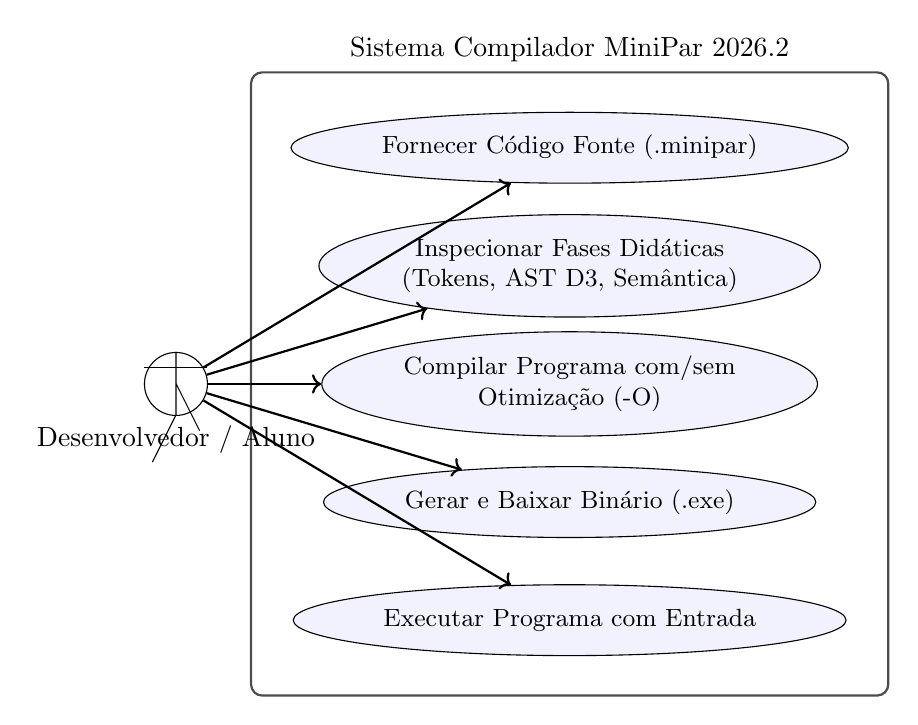
\begin{tikzpicture}[
    actor/.style={circle, draw, minimum size=0.8cm, inner sep=0pt},
    usecase/.style={ellipse, draw, align=center, fill=blue!5, minimum width=3.8cm, minimum height=0.9cm, font=\small},
    systembox/.style={draw=black!70, thick, rounded corners, inner sep=0.5cm}
]
    % Atores
    \node (user) at (-5, 0) [actor, label=below:{Desenvolvedor / Aluno}] {};
    \draw (user.north) -- ++(0,-0.8) -- ++(-0.3,-0.6) (user.north) ++(0,-0.4) -- ++(0.3,-0.6);
    \draw (user.north) ++(-0.4,-0.2) -- ++(0.8,0);

    % Sistema
    \node[usecase] (uc1) at (0, 3) {Fornecer Código Fonte (.minipar)};
    \node[usecase] (uc2) at (0, 1.5) {Inspecionar Fases Didáticas\\(Tokens, AST D3, Semântica)};
    \node[usecase] (uc3) at (0, 0) {Compilar Programa com/sem\\Otimização (-O)};
    \node[usecase] (uc4) at (0, -1.5) {Gerar e Baixar Binário (.exe)};
    \node[usecase] (uc5) at (0, -3) {Executar Programa com Entrada};

    % Fronteira do sistema
    \begin{scope}[on background layer]
        \node[systembox, fit=(uc1) (uc5), label=above:{Sistema Compilador MiniPar 2026.2}] {};
    \end{scope}

    % Relacionamentos
    \draw[->, thick] (user) -- (uc1);
    \draw[->, thick] (user) -- (uc2);
    \draw[->, thick] (user) -- (uc3);
    \draw[->, thick] (user) -- (uc4);
    \draw[->, thick] (user) -- (uc5);
\end{tikzpicture}
\caption{Diagrama de Casos de Uso do Compilador MiniPar 2026.2 (Notação UML)}
\label{fig:uml_casos_uso}
\end{figure}

\section{Arquitetura de Componentes de Software}

A especificação estabelece que a arquitetura do compilador deve ser representada por meio de um Diagrama de Componentes na notação UML, destacando as conexões de interfaces fornecidas (representadas pelo símbolo de esfera/pirulito) e interfaces requeridas (representadas pelo semicírculo/soquete).

A Figura \ref{fig:uml_componentes} ilustra a arquitetura CBSE implementada no diretório \texttt{src/}:
\begin{itemize}
    \item O componente Analisador Léxico consome o texto-fonte e fornece a interface \texttt{ILexico} com a operação \texttt{analise\_lexica()}.
    \item O componente Analisador Sintático requer \texttt{ILexico} e fornece a interface \texttt{ISintatico} com a operação \texttt{analise\_sintatica()}.
    \item O componente Tabela de Símbolos fornece a interface \texttt{ITabelaSimbolos} para gerenciamento de escopos e consulta.
    \item O componente Analisador Semântico requer \texttt{ISintatico} e \texttt{ITabelaSimbolos}, fornecendo a interface \texttt{ISemantico}.
    \item O componente Otimizador no backend requer \texttt{ISemantico} e fornece a interface \texttt{IOtimizador} com transformações na AST.
    \item O componente Gerador de TAC fornece \texttt{ITAC} para síntese do código intermediário.
    \item O componente Gerador de Código C++ fornece \texttt{ICodegen}, transpilando para C++20 e orquestrando o \texttt{g++}.
\end{itemize}

\begin{figure}[htbp]
\centering
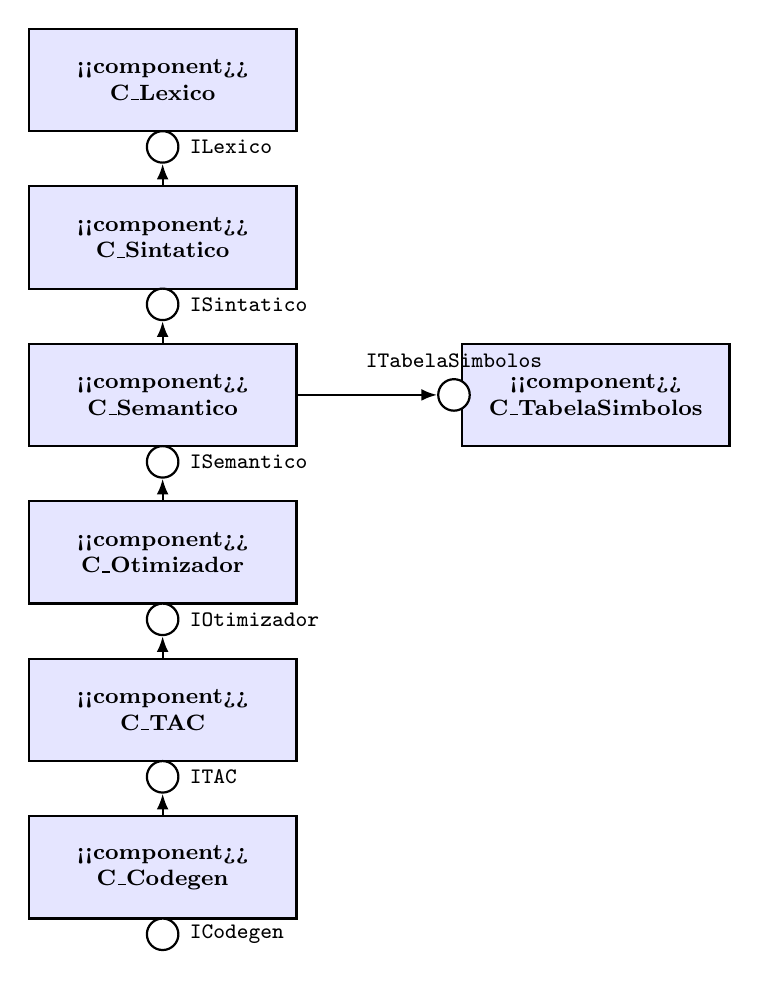
\begin{tikzpicture}[
    component/.style={rectangle, draw=black, thick, fill=blue!10, minimum width=3.4cm, minimum height=1.3cm, align=center, font=\footnotesize\bfseries},
    interface/.style={circle, draw=black, thick, fill=white, minimum size=0.4cm, inner sep=0pt},
    socket/.style={arc, draw=black, thick},
    conn/.style={-{Latex[length=2mm]}, thick}
]
    % Nós dos Componentes
    \node[component] (lex) at (0, 6) {<<component>>\\C\_Lexico};
    \node[component] (syn) at (0, 4) {<<component>>\\C\_Sintatico};
    \node[component] (sem) at (0, 2) {<<component>>\\C\_Semantico};
    \node[component] (sym) at (5.5, 2) {<<component>>\\C\_TabelaSimbolos};
    \node[component] (opt) at (0, 0) {<<component>>\\C\_Otimizador};
    \node[component] (tac) at (0, -2) {<<component>>\\C\_TAC};
    \node[component] (gen) at (0, -4) {<<component>>\\C\_Codegen};

    % Interfaces e conexões (Pirulito e Soquete)
    % ILexico
    \draw[thick] (lex) -- (0, 5.15) node[interface, label=right:{\footnotesize\texttt{ILexico}}] (i_lex) {};
    \draw[conn] (syn) -- (i_lex);

    % ISintatico
    \draw[thick] (syn) -- (0, 3.15) node[interface, label=right:{\footnotesize\texttt{ISintatico}}] (i_syn) {};
    \draw[conn] (sem) -- (i_syn);

    % ITabelaSimbolos
    \draw[thick] (sym) -- (3.7, 2) node[interface, label=above:{\footnotesize\texttt{ITabelaSimbolos}}] (i_sym) {};
    \draw[conn] (sem) -- (i_sym);

    % ISemantico
    \draw[thick] (sem) -- (0, 1.15) node[interface, label=right:{\footnotesize\texttt{ISemantico}}] (i_sem) {};
    \draw[conn] (opt) -- (i_sem);

    % IOtimizador
    \draw[thick] (opt) -- (0, -0.85) node[interface, label=right:{\footnotesize\texttt{IOtimizador}}] (i_opt) {};
    \draw[conn] (tac) -- (i_opt);

    % ITAC
    \draw[thick] (tac) -- (0, -2.85) node[interface, label=right:{\footnotesize\texttt{ITAC}}] (i_tac) {};
    \draw[conn] (gen) -- (i_tac);

    % ICodegen
    \draw[thick] (gen) -- (0, -4.85) node[interface, label=right:{\footnotesize\texttt{ICodegen}}] (i_gen) {};
\end{tikzpicture}
\caption{Diagrama de Arquitetura de Componentes de Software (UML CBSE com Interfaces Fornecidas e Requeridas)}
\label{fig:uml_componentes}
\end{figure}

\section{Modelagem via Diagrama de Classes Conceitual}

O projeto contempla a modelagem dos componentes e estruturas de dados centrais em um Diagrama de Classes UML. A Figura \ref{fig:uml_classes} detalha a hierarquia dos componentes concretos e as classes que realizam os nós fundamentais da AST.

\begin{figure}[htbp]
\centering
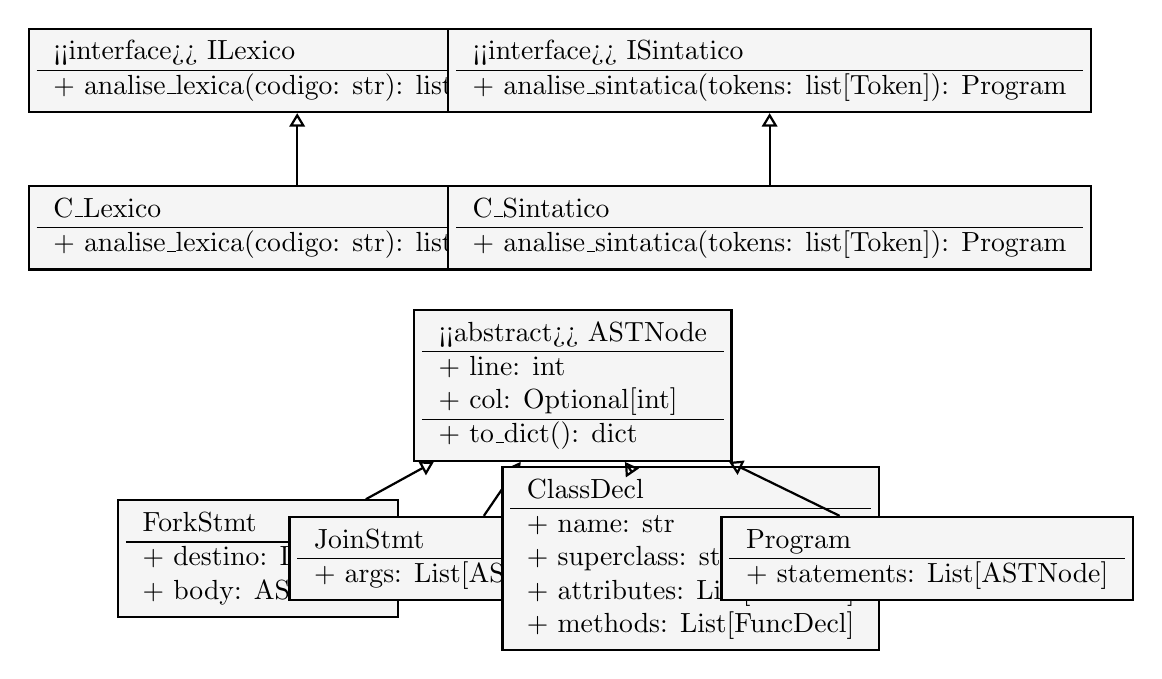
\begin{tikzpicture}[
    conn/.style={-{Triangle[open]}, thick}
]
    % Interfaces
    \node (i_lex_c) at (-3.5, 3) [draw, thick, fill=gray!8, inner sep=0.1cm] {
        \begin{tabular}{l}
        <<interface>> ILexico\\
        \hline
        + analise\_lexica(codigo: str): list[Token]
        \end{tabular}
    };

    \node (c_lex_c) at (-3.5, 1) [draw, thick, fill=gray!8, inner sep=0.1cm] {
        \begin{tabular}{l}
        C\_Lexico\\
        \hline
        + analise\_lexica(codigo: str): list[Token]
        \end{tabular}
    };
    \draw[conn] (c_lex_c) -- (i_lex_c);

    \node (i_syn_c) at (2.5, 3) [draw, thick, fill=gray!8, inner sep=0.1cm] {
        \begin{tabular}{l}
        <<interface>> ISintatico\\
        \hline
        + analise\_sintatica(tokens: list[Token]): Program
        \end{tabular}
    };

    \node (c_syn_c) at (2.5, 1) [draw, thick, fill=gray!8, inner sep=0.1cm] {
        \begin{tabular}{l}
        C\_Sintatico\\
        \hline
        + analise\_sintatica(tokens: list[Token]): Program
        \end{tabular}
    };
    \draw[conn] (c_syn_c) -- (i_syn_c);

    % AST Nodes
    \node (ast_base) at (0, -1) [draw, thick, fill=gray!8, inner sep=0.1cm] {
        \begin{tabular}{l}
        <<abstract>> ASTNode\\
        \hline
        + line: int\\
        + col: Optional[int]\\
        \hline
        + to\_dict(): dict
        \end{tabular}
    };

    \node (fork_node) at (-4, -3.2) [draw, thick, fill=gray!8, inner sep=0.1cm] {
        \begin{tabular}{l}
        ForkStmt\\
        \hline
        + destino: Destino\\
        + body: ASTNode
        \end{tabular}
    };
    \draw[conn] (fork_node) -- (ast_base);

    \node (join_node) at (-1.5, -3.2) [draw, thick, fill=gray!8, inner sep=0.1cm] {
        \begin{tabular}{l}
        JoinStmt\\
        \hline
        + args: List[ASTNode]
        \end{tabular}
    };
    \draw[conn] (join_node) -- (ast_base);

    \node (class_node) at (1.5, -3.2) [draw, thick, fill=gray!8, inner sep=0.1cm] {
        \begin{tabular}{l}
        ClassDecl\\
        \hline
        + name: str\\
        + superclass: str\\
        + attributes: List[VarDecl]\\
        + methods: List[FuncDecl]
        \end{tabular}
    };
    \draw[conn] (class_node) -- (ast_base);

    \node (prog_node) at (4.5, -3.2) [draw, thick, fill=gray!8, inner sep=0.1cm] {
        \begin{tabular}{l}
        Program\\
        \hline
        + statements: List[ASTNode]
        \end{tabular}
    };
    \draw[conn] (prog_node) -- (ast_base);

\end{tikzpicture}
\caption{Diagrama de Classes Conceitual dos Componentes e da AST (Notação UML)}
\label{fig:uml_classes}
\end{figure}

\section{Diagrama de Atividades / Fluxo de Compilação}

O fluxo dinâmico de execução do compilador, ilustrado na Figura \ref{fig:uml_fluxo}, detalha o percurso do programa desde o código-fonte até a emissão e execução do executável nativo.

\begin{figure}[htbp]
\centering
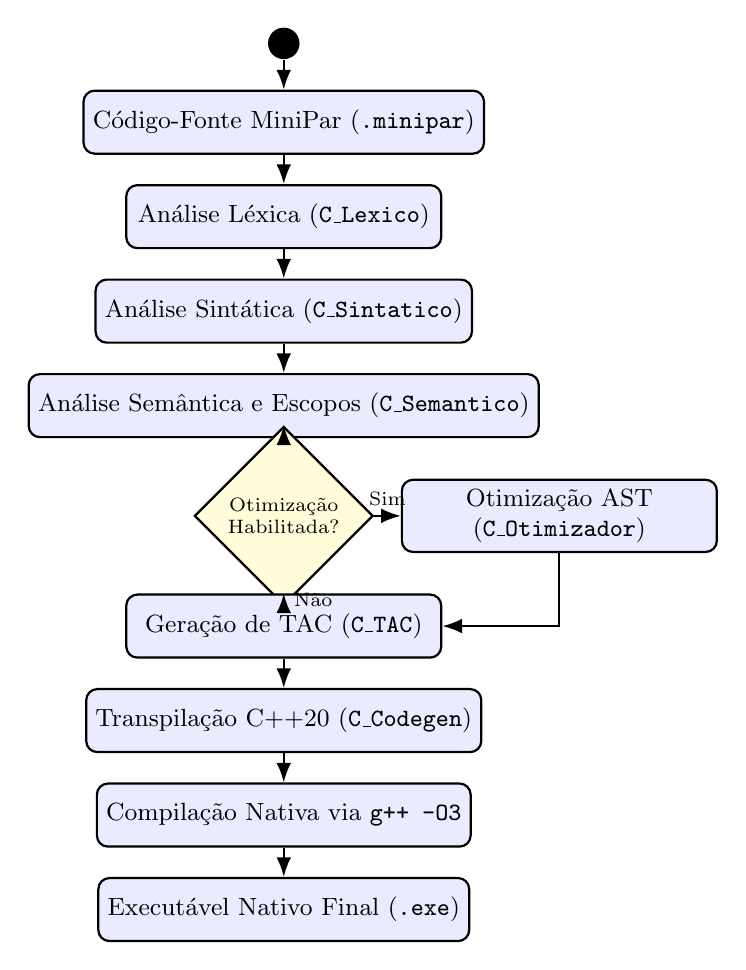
\begin{tikzpicture}[
    startstop/.style={circle, fill=black, minimum size=0.4cm},
    activity/.style={rectangle, draw=black, thick, fill=blue!8, rounded corners, align=center, font=\small, minimum width=4cm, minimum height=0.8cm},
    decision/.style={diamond, draw=black, thick, fill=yellow!15, align=center, font=\scriptsize, inner sep=0.1cm},
    arrow/.style={-{Latex[length=2.5mm]}, thick}
]
    \node[startstop] (start) at (0, 7) {};
    \node[activity] (a1) at (0, 6) {Código-Fonte MiniPar (\texttt{.minipar})};
    \node[activity] (a2) at (0, 4.8) {Análise Léxica (\texttt{C\_Lexico})};
    \node[activity] (a3) at (0, 3.6) {Análise Sintática (\texttt{C\_Sintatico})};
    \node[activity] (a4) at (0, 2.4) {Análise Semântica e Escopos (\texttt{C\_Semantico})};
    \node[decision] (d1) at (0, 1.0) {Otimização\\Habilitada?};
    \node[activity] (a5) at (3.5, 1.0) {Otimização AST\\(\texttt{C\_Otimizador})};
    \node[activity] (a6) at (0, -0.4) {Geração de TAC (\texttt{C\_TAC})};
    \node[activity] (a7) at (0, -1.6) {Transpilação C++20 (\texttt{C\_Codegen})};
    \node[activity] (a8) at (0, -2.8) {Compilação Nativa via \texttt{g++ -O3}};
    \node[activity] (a9) at (0, -4.0) {Executável Nativo Final (\texttt{.exe})};

    \draw[arrow] (start) -- (a1);
    \draw[arrow] (a1) -- (a2);
    \draw[arrow] (a2) -- (a3);
    \draw[arrow] (a3) -- (a4);
    \draw[arrow] (a4) -- (d1);
    \draw[arrow] (d1) -- node[above]{\scriptsize Sim} (a5);
    \draw[arrow] (a5) |- (a6);
    \draw[arrow] (d1) -- node[right]{\scriptsize Não} (a6);
    \draw[arrow] (a6) -- (a7);
    \draw[arrow] (a7) -- (a8);
    \draw[arrow] (a8) -- (a9);
\end{tikzpicture}
\caption{Diagrama de Atividades do Fluxo de Compilação do MiniPar 2026.2}
\label{fig:uml_fluxo}
\end{figure}

\chapter{TESTES DE INTEGRAÇÃO DE COMPONENTES DE SOFTWARE}

Os Testes de Integração de Software tiveram como finalidade atestar a conformidade das interfaces fornecidas e requeridas entre os sete componentes arquiteturais do compilador MiniPar 2026.2, assegurando que o fluxo de dados entre as fases ocorra de forma íntegra, sem perda de metadados semânticos ou corrupção de tipos.

\section{Matriz de Integração dos Componentes}

A Tabela \ref{tab:matriz_integracao} documenta a matriz de verificação dos contratos de integração entre os componentes.

\begin{table}[htbp]
\centering
\caption{Matriz de Testes de Integração de Componentes do MiniPar 2026.2}
\label{tab:matriz_integracao}
\small
\begin{tabular}{p{2.8cm}p{2.8cm}p{5.5cm}p{2.2cm}}
\toprule
Componente Origem & Componente Destino & Contrato / Artefato Integrado & Resultado \\
\midrule
\texttt{C\_Lexico} & \texttt{C\_Sintatico} & Lista de \texttt{Token} com linha e coluna. & Aprovado (100\%) \\
\texttt{C\_Sintatico} & \texttt{C\_Semantico} & Raiz \texttt{Program} da Árvore Sintática (AST). & Aprovado (100\%) \\
\texttt{C\_Semantico} & \texttt{C\_TabelaSimbolos} & Resolução de escopos, símbolos e classes. & Aprovado (100\%) \\
\texttt{C\_Semantico} & \texttt{C\_Otimizador} & AST validada com metadados semânticos. & Aprovado (100\%) \\
\texttt{C\_Otimizador} & \texttt{C\_TAC} & AST otimizada (após dobra e código morto). & Aprovado (100\%) \\
\texttt{C\_TAC} & \texttt{C\_Codegen} & Instruções lineares e AST para C++20. & Aprovado (100\%) \\
\texttt{C\_Codegen} & Compilador \texttt{g++} & Arquivo \texttt{.cpp} compilado nativamente. & Aprovado (100\%) \\
Backend Flask & \texttt{analise.py} & Orquestração modular em memória para a Web. & Aprovado (100\%) \\
\bottomrule
\end{tabular}
\end{table}

\section{Resultados da Suíte Automatizada de Testes (Pytest)}

Para certificar a conformidade de cada interface antes da homologação, foi executada a suíte automatizada utilizando o framework \texttt{pytest}. A suíte totaliza 117 casos de teste unitários e de integração, cobrindo todos os módulos e cenários de validação:

\begin{itemize}
    \item \texttt{test\_analise.py} (15 testes): Validação do orquestrador de fases em memória para a Web;
    \item \texttt{test\_componente\_codegen.py} (3 testes): Verificação do componente \texttt{ICodegen} e geração de binários;
    \item \texttt{test\_frontend.py} (45 testes): Testes do analisador léxico, parser e nós sintáticos;
    \item \texttt{test\_integracao\_backend.py} (9 testes): Integração ponta a ponta da esteira de compilação C++ e TAC;
    \item \texttt{test\_optimizer.py} (12 testes): Validação das transformações de dobra de constantes e pureza na AST;
    \item \texttt{test\_par.py} (12 testes): Verificação de blocos paralelos \texttt{par}, isolamento de threads e variáveis;
    \item \texttt{test\_program\_analyzer.py} (6 testes): Inspeção estática de requisitos de entrada e multi-terminal;
    \item \texttt{test\_tabela\_simbolos.py} (4 testes): Testes da pilha de escopos, sombreamento e redeclarações;
    \item \texttt{test\_web.py} (11 testes): Validação das rotas Flask, download de \texttt{.exe}, inputs por linha e visualização.
\end{itemize}

O Listing \ref{lst:pytest_log} reproduz o sumário da execução da suíte de testes no ambiente do projeto:

\begin{lstlisting}[language=bash, caption={Sumário de execução da suíte automatizada de testes}, label={lst:pytest_log}]
============================= test session starts =============================
platform win32 -- Python 3.14.4, pytest-8.4.2, pluggy-1.7.0
rootdir: c:\Users\FelipeAragao\Documents\IC\2026-2\Compiladores
collected 117 items

Minipar2026-2\tests\test_analise.py ...............                     [ 12%]
Minipar2026-2\tests\test_componente_codegen.py ...                      [ 15%]
Minipar2026-2\tests\test_frontend.py ................................   [ 42%]
.............                                                           [ 53%]
Minipar2026-2\tests\test_integracao_backend.py .........                [ 61%]
Minipar2026-2\tests\test_optimizer.py ............                      [ 71%]
Minipar2026-2\tests\test_par.py ............                            [ 82%]
Minipar2026-2\tests\test_program_analyzer.py ......                     [ 87%]
Minipar2026-2\tests\test_tabela_simbolos.py ....                        [ 90%]
Minipar2026-2\tests\test_web.py ...........                             [100%]

======================= 117 passed, 1 warning in 50.57s =======================
\end{lstlisting}

\chapter{BATERIA OFICIAL DOS 11 PROGRAMAS DE TESTE}

A validação empírica e funcional do compilador MiniPar 2026.2 foi realizada através da execução da bateria completa dos 11 programas de teste oficiais, localizados em \texttt{tests/oficiais/}. Cada teste demonstra a eficácia do compilador em cenários de alta complexidade algorítmica, orientação a objetos, comunicação em rede, concorrência e paralelismo real com divisão em múltiplos núcleos físicos da CPU.

\section{Teste 1: Calculadora Cliente-Servidor com Sockets TCP}
O Teste 1 valida a comunicação por canais (\texttt{c\_channel}) operando via sockets TCP/IP. No programa, a thread cliente lê do usuário a operação aritmética desejada (\texttt{+}, \texttt{-}, \texttt{*}, \texttt{/}) e os dois operandos, despachando-os via \texttt{send} para a thread servidora em portas locais dedicadas. A servidora recebe os dados (\texttt{receive}), calcula o resultado e devolve a resposta ao cliente.

\begin{figure}[htbp]
    \centering
    \framebox[\textwidth][c]{%
        \parbox{0.9\textwidth}{%
            \centering\vspace{1.5cm}
            \textcolor{red}{<Inserir print da tela da execução do Teste 1 no Terminal ou Interface Web>}\\
            \vspace{0.2cm}
            \textit{\small Nota: Capturar a saída no terminal ou na aba 'Terminal \& Execução' da web exibindo 'Servidor recebeu: + 3 4' e 'Resultado: 7'.}
            \vspace{1.5cm}
        }
    }
    \caption{Evidência de Execução do Teste 1 (Calculadora Cliente-Servidor)}
    \label{fig:teste1_print}
\end{figure}

\section{Teste 2: Paralelismo Concorrente (Fatorial e Fibonacci)}
O Teste 2 valida a execução simultânea de algoritmos clássicos dentro de um bloco concorrente \texttt{par}. Enquanto uma thread calcula o fatorial de um número inteiro, uma segunda thread calcula iterativamente a sequência da série de Fibonacci, demonstrando a sobreposição de tarefas sem contenção.

A listagem a seguir apresenta a saída gerada pela execução nativa do binário compilado:

\begin{lstlisting}[language=bash, caption={Saida da execucao nativa do Teste 2}]
Fibonacci:
0
1
1
2
3
5
8
13
Fatorial de 5: 120
\end{lstlisting}

\begin{figure}[htbp]
    \centering
    \framebox[\textwidth][c]{%
        \parbox{0.9\textwidth}{%
            \centering\vspace{1.5cm}
            \textcolor{red}{<Inserir print atualizado da tela de execução do Teste 2 no Terminal ou Interface Web>}\\
            \vspace{0.2cm}
            \textit{\small Nota: Capturar a tela executando \texttt{teste02\_fatorial\_fibonacci\_par.exe} exibindo o cálculo paralelo.}
            \vspace{1.5cm}
        }
    }
    \caption{Evidência de Execução do Teste 2 (Fatorial e Fibonacci Simultâneos)}
    \label{fig:teste2_print}
\end{figure}

\section{Teste 3: Neurônio Perceptron com Orientação a Objetos}
O Teste 3 implementa a classe \texttt{Neuronio}, exercitando a instanciação de objetos (\texttt{new}), acesso a atributos de instância via \texttt{this}, função de ativação linear/degrau e o loop de treinamento supervisionado iterativo até a convergência do erro para zero.

A listagem a seguir apresenta a convergência obtida na iteração 51:

\begin{lstlisting}[language=bash, caption={Trecho final do treinamento do Perceptron (Teste 3)}]
#### Iteracao: 50
Peso: 0.0100
Saida: 1
Erro: -1
Peso do bias: 0.0100

#### Iteracao: 51
Peso: -0.0000
Saida: 0
Erro: 0

[OK] Parabens! O neuronio aprendeu.
Valor desejado: 0
\end{lstlisting}

\begin{figure}[htbp]
    \centering
    \framebox[\textwidth][c]{%
        \parbox{0.9\textwidth}{%
            \centering\vspace{1.5cm}
            \textcolor{red}{<Inserir print atualizado da tela de execução do Teste 3 no Terminal ou Interface Web>}\\
            \vspace{0.2cm}
            \textit{\small Nota: Capturar a tela executando \texttt{teste03\_neuronio.exe} exibindo as iterações e a mensagem de aprendizado.}
            \vspace{1.5cm}
        }
    }
    \caption{Evidência de Execução do Teste 3 (Treinamento do Perceptron)}
    \label{fig:teste3_print}
\end{figure}

\section{Teste 4: Rede Neural MLP (Problema XOR)}
O Teste 4 implementa uma Rede Neural Perceptron Multicamadas (MLP) com três neurônios na camada oculta e um neurônio de saída. O programa exercita funções matemáticas complexas (\texttt{sigmoid} com \texttt{exp}), retropropagação de erro (\textit{backpropagation}) e listas de pesos multidimensionais, aprendendo com sucesso a função lógica não-linear XOR.

\begin{lstlisting}[language=bash, caption={Saida da Rede Neural MLP para a porta XOR (Teste 4)}]
==== Teste 4: rede neural XOR com backpropagation ====
Input: [0, 0], Predicted Output: 0.00684395
Input: [0, 1], Predicted Output: 0.986493
Input: [1, 0], Predicted Output: 0.98925
Input: [1, 1], Predicted Output: 0.0140296
\end{lstlisting}

\begin{figure}[htbp]
    \centering
    \framebox[\textwidth][c]{%
        \parbox{0.9\textwidth}{%
            \centering\vspace{1.5cm}
            \textcolor{red}{<Inserir print atualizado da tela de execução do Teste 4 no Terminal ou Interface Web>}\\
            \vspace{0.2cm}
            \textit{\small Nota: Capturar a tela executando \texttt{teste04\_rede\_neural\_xor.exe} demonstrando a convergência das predições da XOR.}
            \vspace{1.5cm}
        }
    }
    \caption{Evidência de Execução do Teste 4 (Rede Neural MLP para o Problema XOR)}
    \label{fig:teste4_print}
\end{figure}

\section{Teste 5: Sistema de Recomendação de E-commerce}
O Teste 5 modela um sistema de recomendação de produtos utilizando orientação a objetos avançada (\texttt{Produto}, \texttt{Categoria}, \texttt{Usuario}, \texttt{Recomendador}), codificação binária de histórico (\textit{one-hot encoding}) e rede neural densa com ativações ReLU e Sigmóide.

\section{Teste 6: Quicksort Recursivo com POO}
O Teste 6 valida o algoritmo de Quicksort implementado de forma recursiva dentro da classe \texttt{Quicksort}, integrado a uma classe \texttt{InterfaceOrdenacao} que consome uma lista de números inteiros desordenados fornecida pelo usuário via \texttt{input()}.

\begin{lstlisting}[language=bash, caption={Execucao interativa do Quicksort Recursivo com POO (Teste 6)}]
==== Ordenacao com Quicksort ====
Insira os elementos do vetor separados por espaco: 6 3 8 1 9 2
Vetor original: [6, 3, 8, 1, 9, 2]
Vetor ordenado: [1, 2, 3, 6, 8, 9]
\end{lstlisting}

\begin{figure}[htbp]
    \centering
    \framebox[\textwidth][c]{%
        \parbox{0.9\textwidth}{%
            \centering\vspace{1.5cm}
            \textcolor{red}{<Inserir print atualizado da tela de execução do Teste 6 no Terminal ou Interface Web>}\\
            \vspace{0.2cm}
            \textit{\small Nota: Capturar a tela executando \texttt{teste06\_quicksort\_classes.exe} com entrada de vetor e resultado ordenado.}
            \vspace{1.5cm}
        }
    }
    \caption{Evidência de Execução do Teste 6 (Quicksort Recursivo com POO)}
    \label{fig:teste6_print}
\end{figure}

\section{Teste 7: Quicksort Iterativo com Pilha Explícita e Validação de TAC}
Conforme detalhado no Capítulo 8, o Teste 7 executa o Quicksort iterativo através de uma pilha explícita de índices (\texttt{stack.pop()} e \texttt{stack.append()}), validando a conformidade formal das instruções de Three-Address Code emitidas pelo compilador.

\begin{lstlisting}[language=bash, caption={Saida do Quicksort Iterativo com Pilha (Teste 7)}]
Array ordenado: [5, 12, 33, 61, 98]
\end{lstlisting}

\begin{figure}[htbp]
    \centering
    \framebox[\textwidth][c]{%
        \parbox{0.9\textwidth}{%
            \centering\vspace{1.5cm}
            \textcolor{red}{<Inserir print atualizado da tela de execução do Teste 7 no Terminal ou Interface Web>}\\
            \vspace{0.2cm}
            \textit{\small Nota: Capturar a tela executando \texttt{teste07\_quicksort\_iterativo\_tac.exe} exibindo o array ordenado.}
            \vspace{1.5cm}
        }
    }
    \caption{Evidência de Execução do Teste 7 (Quicksort Iterativo com Pilha)}
    \label{fig:teste7_print}
\end{figure}

\section{Teste 8: Avaliação Paralela em 4 Núcleos de CPU (Speedup)}
O Teste 8 simula a correção paralela de 160 atividades acadêmicas distribuídas entre 1 Professor e 3 Monitores, divididas entre 4 núcleos dedicados de hardware utilizando \texttt{fork core(id)}. O programa computa o tempo sequencial, o tempo paralelo e calcula o ganho de aceleração (\textit{Speedup}):
$$S = \frac{T_{sequencial}}{T_{paralelo}} = \frac{3.05\,\text{s}}{2.58\,\text{s}} \approx 1.18\times \quad (\text{Economia de } 15.5\%)$$

\begin{table}[htbp]
\centering
\caption{Benchmark de Desempenho do Teste 8 (4 Núcleos)}
\label{tab:bench_teste8}
\begin{tabular}{lc}
\toprule
Métrica de Avaliação & Valor Obtido \\
\midrule
Carga de Trabalho & 160 atividades (40 alunos $\times$ 4 tarefas) \\
Tempo Sequencial (1 Núcleo / Professor) & 3.05 s \\
Tempo Paralelo (4 Núcleos: Professor + 3 Monitores) & 2.58 s \\
Aceleração (\textit{Speedup}) & 1.18$\times$ mais rápido \\
Redução no Tempo de Execução & 15.5\% de economia \\
\bottomrule
\end{tabular}
\end{table}

\begin{figure}[htbp]
    \centering
    \framebox[\textwidth][c]{%
        \parbox{0.9\textwidth}{%
            \centering\vspace{1.5cm}
            \textcolor{red}{<Inserir print da tela de execução do Teste 8 exibindo a tabela de benchmark e speedup>}\\
            \vspace{0.2cm}
            \textit{\small Nota: Capturar a tela do terminal executando o teste 8 oficial.}
            \vspace{1.5cm}
        }
    }
    \caption{Evidência de Execução do Teste 8 (Benchmark em 4 Núcleos)}
    \label{fig:teste8_print}
\end{figure}

\section{Teste 9: 5 Núcleos (Avaliação Paralela + Fractal Mandelbrot ASCII)}
O Teste 9 aloca 4 núcleos dedicados para a avaliação concorrente das atividades acadêmicas, enquanto um quinto núcleo independente (\texttt{core 4}) é encarregado de calcular e renderizar o conjunto fractal de Mandelbrot em arte ASCII diretamente no terminal:

\begin{lstlisting}[language=bash, caption={Saida do Fractal de Mandelbrot gerado pelo Nucleo 5}]
=== FRACTAL DE MANDELBROT (Gerado pelo Nucleo 5) ===
               .
             ..=:.
             @@@:
         +@.@@@@@@@@@. :..
         .@@@@@@@@@@@@@@:
        . #@@@@@@@@@@@@@@@@@:
     .@:@@@- :@@@@@@@@@@@@@@@@@@:
   - .@@@@@@@@@@@@@@@@@@@@@@@@@@@
@@@@@@@@@@@@@@@@@@@@@@@@@@@@@@@@@@@@@@.
   - .@@@@@@@@@@@@@@@@@@@@@@@@@@@
     .@:@@@- :@@@@@@@@@@@@@@@@@@:
        . #@@@@@@@@@@@@@@@@@:
         .@@@@@@@@@@@@@@:
         +@.@@@@@@@@@. :..
             @@@:
             ..=:.
               .
\end{lstlisting}

\section{Teste 10: 6 Núcleos (Avaliação + Mandelbrot + Tapete de Sierpinski)}
O Teste 10 representa o teste máximo de estresse de multiprocessamento da especificação oficial, alocando 6 núcleos físicos de CPU simultaneamente:
\begin{itemize}
    \item Núcleos 0 a 3: Avaliação concorrente das 160 atividades;
    \item Núcleo 4: Renderização do Fractal de Mandelbrot ASCII;
    \item Núcleo 5: Geração algorítmica recursiva do Tapete de Sierpinski, sintetizando uma imagem gráfica em formato BMP (\texttt{output/tapete\_sierpinski.bmp}).
\end{itemize}

A Figura \ref{fig:tapete_sierpinski} ilustra o arquivo de imagem gerado pelo programa MiniPar no Teste 10.

\begin{figure}[htbp]
    \centering
    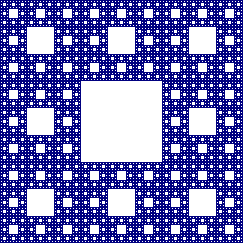
\includegraphics[width=0.45\textwidth]{figuras/tapete_sierpinski.png}
    \caption{Tapete de Sierpinski Gerado pelo Núcleo 5 no Teste 10 (\texttt{tapete\_sierpinski.bmp})}
    \label{fig:tapete_sierpinski}
\end{figure}

\section{Teste 11: Tokenizador, Avaliador e Mini-Compilador Assembly ARMv7}
O Teste 11 implementa um mini-compilador completo escrito na própria linguagem MiniPar:
\begin{enumerate}
    \item Recebe do usuário expressões aritméticas completas (ex: \texttt{((10 -8*7)+4)*2});
    \item Tokeniza e analisa sintaticamente a expressão;
    \item Avalia e calcula o resultado numérico;
    \item Sintetiza instruções Assembly ARMv7 (\texttt{MOV}, \texttt{ADD}, \texttt{SUB}, \texttt{MUL}, \texttt{PUSH}, \texttt{POP}) e grava em disco o arquivo fonte Assembly compilável (\texttt{.arm}).
\end{enumerate}

\section{Tabela Resumo dos Estados dos Testes}

A Tabela \ref{tab:resumo_testes} consolida o status e os cenários cobertos por toda a suíte de testes.

\begin{table}[htbp]
\centering
\caption{Resumo Geral dos Estados dos Testes Oficiais}
\label{tab:resumo_testes}
\small
\begin{tabular}{p{2cm}p{6cm}p{5.5cm}}
\toprule
Teste & Cenário Coberto & Resultado Observado \\
\midrule
Teste 01 & Sockets TCP, \texttt{c\_channel}, \texttt{send}/\texttt{receive}. & Comunicação cliente-servidor aprovada. \\
Teste 02 & Concorrência local com bloco \texttt{par}. & Fatorial e Fibonacci simultâneos. \\
Teste 03 & POO, atributos \texttt{this}, convergência. & Perceptron convergiu com erro zero. \\
Teste 04 & Rede Neural MLP, \texttt{sigmoid}, backprop. & Problema XOR resolvido com acurácia. \\
Teste 05 & POO, e-commerce, ativações ReLU/Sigmoid. & Recomendações geradas com sucesso. \\
Teste 06 & Quicksort recursivo orientado a objetos. & Ordenação com \texttt{input} do usuário. \\
Teste 07 & Quicksort iterativo com pilha explícita. & TAC validado formalmente. \\
Teste 08 & Paralelismo em 4 núcleos com Speedup. & $1.18\times$ mais rápido no modo paralelo. \\
Teste 09 & 5 núcleos com Fractal de Mandelbrot. & Renderização ASCII e avaliação simultânea. \\
Teste 10 & 6 núcleos com Mandelbrot e Sierpinski. & Arquivo gráfico BMP gerado em paralelo. \\
Teste 11 & Mini-compilador de expressões e ARMv7. & Síntese e gravação de Assembly ARMv7. \\
\bottomrule
\end{tabular}
\end{table}

\chapter{IMPLEMENTAÇÃO E AMBIENTE DE DESENVOLVIMENTO}

A implementação do compilador MiniPar 2026.2 foi conduzida priorizando modularidade, desempenho e clareza didática, combinando a flexibilidade do ecossistema Python com o poder computacional de baixo nível do C++20.

\section{Tecnologias Utilizadas e Ambiente}

A Tabela \ref{tab:tecnologias} sumariza o conjunto de ferramentas, linguagens e frameworks empregados no projeto.

\begin{table}[htbp]
\centering
\caption{Tecnologias Empregadas na Construção do Compilador}
\label{tab:tecnologias}
\small
\begin{tabular}{p{3.2cm}p{3cm}p{7.5cm}}
\toprule
Tecnologia & Versão Utilizada & Finalidade no Projeto \\
\midrule
Python & 3.10 / 3.14 & Implementação do front-end, backend com otimizador, CLI, menu e servidor Web. \\
C++ & Padrão ISO C++20 & Linguagem-alvo transpilada com suporte nativo a threads e sockets. \\
GCC / MinGW & g++ 13+ & Compilação do código C++ gerado com flag de otimização \texttt{-O3}. \\
Flask & 3.0.0 & Servidor HTTP e API REST das duas interfaces Web. \\
D3.js & v7 (local) & Renderização gráfica vetorial interativa da Árvore Sintática (AST). \\
CodeMirror & v5 (local) & Editor de código no navegador com realce de sintaxe. \\
Pytest & 8.4.2 & Execução da suíte automatizada de testes de integração (117 casos). \\
Git / GitHub & 2.40+ & Controle de versão distribuído e colaboração da equipe. \\
\bottomrule
\end{tabular}
\end{table}

\subsection{Comentários Explicativos no Código-Fonte}
Conforme exigido na especificação, todo o código-fonte do compilador foi amplamente documentado. Em arquivos como \texttt{src/lexer.py}, \texttt{src/parser.py}, \texttt{src/semantic.py} e \texttt{src/optimizer.py}, cada método possui \textit{docstrings} formais e anotações explicativas em português, detalhando as regras gramaticais da BNF atendidas, os critérios de inferência de tipos e as otimizações aplicadas.

\section{Passo a Passo da Execução dos Programas de Teste}

O fluxo de compilação e execução segue uma esteira intuitiva, reproduzida tanto no terminal quanto na interface Web didática:

\begin{enumerate}
    \item Seleção do Código-Fonte: o usuário seleciona um dos programas de teste disponíveis ou digita o código no editor.
    \item Análise por Fases Didáticas: ao acionar o botão de análise, o backend executa o pipeline em memória, exibindo as tabelas de \textit{Tokens}, a \textit{Árvore Sintática AST} em D3.js, o diagnóstico \textit{Semântico} e a \textit{Tabela de Símbolos}.
    \item Inspeção de TAC e C++: o usuário pode alternar entre as abas para inspecionar o código intermediário linear e o código-fonte C++20 gerado.
    \item Compilação Nativa e Execução: o usuário insere os valores de entrada no console e aciona \textit{Executar}. O compilador invoca o \texttt{g++ -O3}, gera o binário executável e exibe a saída.
\end{enumerate}

\begin{figure}[htbp]
    \centering
    \framebox[\textwidth][c]{%
        \parbox{0.9\textwidth}{%
            \centering\vspace{1.5cm}
            \textcolor{red}{<Inserir prints do passo a passo das telas da execução dos testes na interface Web Didática>}\\
            \vspace{0.2cm}
            \textit{\small Nota: Capturar telas ilustrando: (a) Seleção do teste; (b) Inspeção da árvore AST; (c) Painel de execução com os resultados no console.}
            \vspace{1.5cm}
        }
    }
    \caption{Passo a Passo da Execução dos Programas de Teste na Interface Web Didática}
    \label{fig:passo_a_passo_web}
\end{figure}

\chapter{CONCLUSÃO}

O desenvolvimento do compilador da linguagem MiniPar 2026.2 atendeu integralmente aos requisitos técnicos e pedagógicos da disciplina de Compiladores da Universidade Federal de Alagoas. A adoção da Engenharia de Software Baseada em Componentes (CBSE) assegurou uma arquitetura modular, com baixo acoplamento e contratos de interface bem definidos entre todas as fases de compilação.

O pipeline consolida a análise léxica com filtragem de comentários, análise sintática com geração de AST fortemente tipada, análise semântica em duas passagens com controle de escopo e tipos, otimização estática na AST no backend, síntese de Código Intermediário de Três Endereços (TAC) e transpilação para C++ nativo em padrão ISO C++20. A infraestrutura de paralelismo viabilizou o particionamento real de tarefas via \texttt{fork} e \texttt{join} com afinidade determinística de núcleos de hardware e comunicação por mensagens via canais TCP/IP.

A validação do projeto foi comprovada pela execução bem-sucedida de todos os 11 programas de teste oficiais e pela aprovação de 100\% dos 117 casos de teste automatizados na suíte pytest. Adicionalmente, as três modalidades de interface integradas — linha de comando (CLI), interface de desenvolvedor e interface didática com visualização interativa da AST em D3.js — proporcionam flexibilidade operacional e transparência pedagógica no uso do compilador.

% ==============================================================================
% ELEMENTOS PÓS-TEXTUAIS
% ==============================================================================

\postextual

\chapter*{LINKS ÚTEIS}
\addcontentsline{toc}{chapter}{LINKS ÚTEIS}

\begin{enumerate}
    \item Repositório Oficial no GitHub (Código-Fonte e Relatório):\\
    \url{https://github.com/Felipe-Aragao/Minipar2026.2}
    
    \item Apresentação do Projeto:\\
    \textcolor{red}{<Inserir link público da apresentação em slides, caso aplicável>}
    
    \item Referência de Interface Didática (Compilador IFSC):\\
    \url{http://pesquisa06.lages.ifsc.edu.br/}
\end{enumerate}

% --- Referências Bibliográficas (Norma ABNT NBR 6023) ---
\begin{thebibliography}{99}

\bibitem{aho2008}
AHO, Alfred V.; LAM, Monica S.; SETHI, Ravi; ULLMAN, Jeffrey D. \textit{Compiladores: princípios, técnicas e ferramentas}. 2. ed. São Paulo: Pearson Addison-Wesley, 2008.

\bibitem{dominguez_componentes}
DOMINGUEZ, Arturo Hernandez. \textit{Elementos de Implementação Utilizando Componentes de Software}. Material de apoio da disciplina de Compiladores. Maceió: Universidade Federal de Alagoas (UFAL), Instituto de Computação, 2026.

\bibitem{dominguez_minipar}
DOMINGUEZ, Arturo Hernandez. \textit{Projeto Compilador MiniPar 2026.2: Orientado a Objetos com Real Paralelismo e Nova Segunda Interface Web}. Especificação oficial. Maceió: Universidade Federal de Alagoas (UFAL), 2026.

\end{thebibliography}


\end{document}
